\documentclass[12pt, a4paper, titlepage]{article}
\usepackage{url}
% font size could be 10pt (default), 11pt or 12 pt
% paper size coulde be letterpaper (default), legalpaper, executivepaper,
% a4paper, a5paper or b5paper
% side coulde be oneside (default) or twoside 
% columns coulde be onecolumn (default) or twocolumn
% graphics coulde be final (default) or draft 
%
% titlepage coulde be notitlepage (default) or titlepage which 
% makes an extra page for title 
% 
% paper alignment coulde be portrait (default) or landscape 
%
% equations coulde be 
%   default number of the equation on the rigth and equation centered 
%   leqno number on the left and equation centered 
%   fleqn number on the rigth and  equation on the left side
%
\usepackage[
  textwidth=17cm,
  outer=2cm,
  textheight=45\baselineskip,
  headheight=\baselineskip,
  includehead=false,% Default
  heightrounded,
]{geometry}
\usepackage{fancyhdr}
\usepackage{graphicx}\DeclareGraphicsExtensions{.ps,.eps}

\pagestyle{fancy}
\bibliographystyle{acm}
\fancyhead{}
\fancyhead[LO]{\leftmark}
\fancyhead[RE]{\rightmark}

\usepackage{float}
\usepackage{booktabs}
\usepackage{hyperref}

\usepackage{xcolor}
\usepackage{fancybox}

\usepackage[most]{tcolorbox}
\definecolor{ShadowColor}{RGB}{30,150,190}

%\usepackage[light]{draftcopy}

\providecommand{\versionnumber}{DRAFT 0.1}


\title{AppCoins\\ Distributed and Trusted App-based Transactions Platform}
\author{\small Paulo Trezentos  \\
  {\em  ISCTE / Aptoide}  \\
  \and 
\small  Diogo Pires \\
  {\em Aptoide} \\
  \and
  Aptoide Team
  }





\date{\today\\\normalsize Version \versionnumber} 
% \date{\today} date coulde be today 
% \date{25.12.00} or be a certain date
% \date{ } or there is no date 
\begin{document}
% Hint: \title{what ever}, \author{who care} and \date{when ever} could stand 
% before or after the \begin{document} command 
% BUT the \maketitle command MUST come AFTER the \begin{document} command! 
\maketitle


\begin{abstract}

There are today, in 2017, 2.1 billion smartphone users in the world and the number is expected to grow to  4 billion in 2020. To install apps and games, those mobile users use app stores. An app store is the distribution channel between the developer and the user. App stores generate more that \$77 billion yearly in gross revenue.  However, they seem to be incapable of solving the most basic issues that harm the app store experience: inaccessibility of in-app purchases, advertising model intermediation, malware and lack of innovation.

The reasons are diverse: inadequacy of payment models to emergent countries and younger generations, no trust between the actors of the ecosystem and lack of standardisation defining clear interfaces and enabling market free entry for new players.

AppCoins is an open and distributed protocol for App Stores. It proposes to move to the blockchain three of the most critical flows of app stores: advertising, in-app billing and developers approval. By redesigning the transactions inside an App Store, creates efficiencies by disintermediation and redistributes the value released in a way that create incentives for the AppCoins supported stores dissemination.

The design of the protocol received contributions of players in the app store industry as well as the blockchain community, aiming to change the apps distribution in 3 ways: ``open'' with open standards that enables trust and privacy, ``circular'' where the value created in a transaction is not drained by intermediaries but flows in a virtuous loop, and ``shared'' where knowledge and open source code benefits every member of the community.

The bootstrap of the protocol will be accomplished in the next 12 months, using the 142 million yearly unique active users of Aptoide app store user base, and leveraging the tokens not distributed in the ICO to incentivise developers, OEMs and users to use technology powered by the protocol.

The goal is that by 2022, in five years time, 1.3 billion people use an AppCoins supported app store.


\end{abstract}

%\tableofcontents % create a table of contens 

\tableofcontents




\section{Introduction and Problem Statement}
\label{sec: introduction}

\subsection{Motivation}

%XXX general idea. maybe introduce introduce a table of abbreviations?

% (Give a brief overview of App Store ecosystem and intermediaries.) 

% (Explaining the problem for each of the 3 main flows. Problem of double attribution, problem of refutation,....)

Aptoide app store was used in 142 million unique devices in 2016 by the user to install at least one app. Although the Aptoide brand may, or not, be familiar to you before reading this white paper, every one in five kids in the world between the ages of 16 and 25 uses Aptoide. In certain countries - like Brazil or Mexico\footnote{Aptoide Top 5 countries: Brazil, Mexico, US, India, Italy} - that is one in three kids using it. 

Over this incredible journey to earn the trust of Aptoide users, without any payed acquisition, we discovered that app stores can be much more. The app discovery can be much better. The financial transactions, like advertising and in-app purchases, can be much more eficient. The sharing can be much more powerful. 

The current state does not benefit the developers or the user. It only benefits Google and Apple. In a closed market, they can impose margins and their own distribution rules.

\medskip

The proposed protocol in this document is a call to the community. Is a call to developers, to other app stores, to users. Is a call to work together toward a free-entry app store market. A market that unclocks the world of in-app purchases to billions of users. A market that benefits the talented developers providing significant revenue and transparent ways to reach their users. AppCoins proposes a market where app stores compete by innovation and service.

As open source and community helped us to reach 100 million users in 4 years, we are certain that {\em blockchain} is the technology that will enable this revolution, provinding trust and transparency.

If you share this vision with us, join us in this new journey, collaborating in the protocol, developing open source software and spreading the word. Changing the app store ecosystem and breaking monopolies.


\medskip

\subsection{History}

App stores are a distribution channel between the developer and the end user. Although software distribution exists since there is software development, the current model of smartphone became popular with the launch of Apple's App Store in July 2008 and with its pre-load in iPhone 3G.

In the same year, but later in August 2008, Google announced the launch of Android Market \cite{wiki:market}, the app store for Android.

These initial app stores followed a centralised model where one entity is responsible for assuring the core features of software distribution: file delivery, app discovery, financial transactions and app approval. Centralisation in the context of app stores means no transparency and being closed source. As the smartphone user base grew, the centralised model started to show severe flaws. The flaws and problems identified are strongly related with the existent model: a lack of trust and economical efficiency.

Non-transparency means app stores can avoid disclosing the reasoning behind their decisions. An example is censoring apps that are seen by them as competitors or that do not follow the rules set by them. On the other hand, being closed source creates the possibility to hide processes from users, such as collecting user data (e.g. user age, preferences, apps installed, etc) for other purposes.

By not being transparent, app stores do not earn the trust among the different stakeholders: developers, advertisers, users and OEM manufacturers. By being centralised, they cannot benefit from a shared and crowdsourcing economy. Being closed source and hiding data, they do not promote competition and innovation.

The AppCoins protocol covers three core app store use cases:

\begin{itemize}
\item {\bf Advertising inside the app store}: The transactional flow where a developer pays for a user to install their app or game. There are different advertising models depending on the action that triggers the actual payment of the Ad: CPI (Cost per Installation), CPA (Cost per Action), CPM (Cost per Thousand Impressions) and others. There are different technologies and platforms to support it: Ad networks, Exchanges and RTB (Real Time Bidding).
\item {\bf In-App Purchase}: When there is something that the user wants to buy inside the app or game, like gems or unlock levels, the purchase mechanism is done through the app store. To enable those transactions, the developer has to integrate the SDK from the app store or to use the app store API.
\item {\bf App approval}: In order for the app to be available, the developer has to go through an approval process where the app store screens the app through automatic tools like anti-virus, anti-malware tools and static and dynamic code analysis platforms. Some app stores also manually test the app.
\end{itemize}


\begin{figure}[!ht]
\centering
%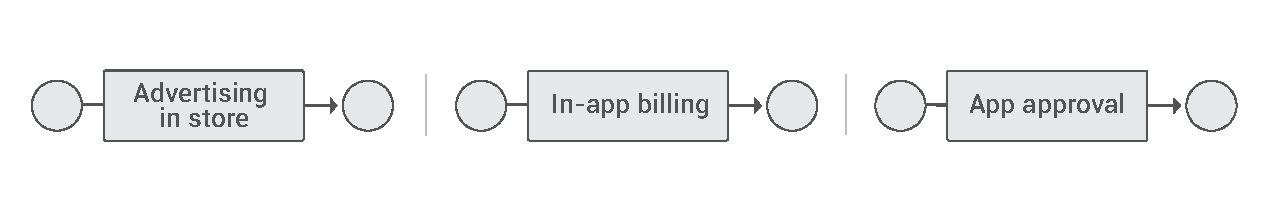
\includegraphics[width=11cm]{diagrams/current_flows.eps}
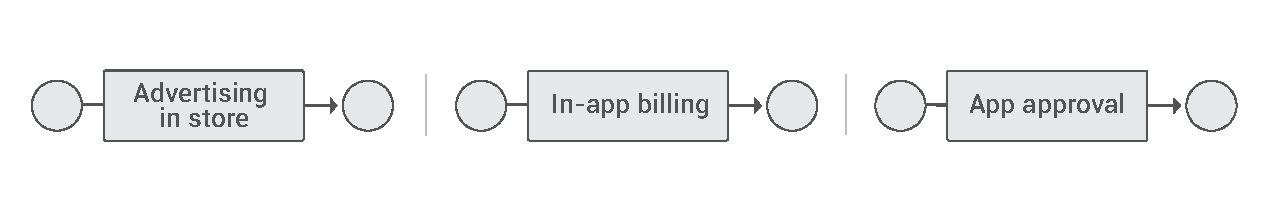
\includegraphics[width=\textwidth]{diagrams/current_flows.eps}
\caption{Individual existent core flows in app stores.}
\label{fig:exist_flows}
\end{figure}




In the next sub-sections, we'll analyse each of the above flows and the main problems faced today.

\subsection{Advertising}
\label{subsec:intro_ads}


Currently, the three flows presented in Figure \ref{fig:exist_flows} do not have any interaction among them. They are isolated and handled by different app store teams. The resources and information generated by one flow are not reused by the others. The intermediaries are many and were introduced to solve the lack of trust and the need to integrate with different players in a fragmented market.  

% XXX which flows: the flows cannot be easily identified
% XXX The resources ... sentence seems to be redundant.

In the next sub-sections, we will analyse each of the flows individually and the main problems faced today.

For a developer or a publisher, the most natural place to advertise an application or game is where the users are looking for that kind of content: the app store.

\begin{figure}[!ht]
\centering
%\includegraphics[width=11cm]{diagrams/current_flows.png}
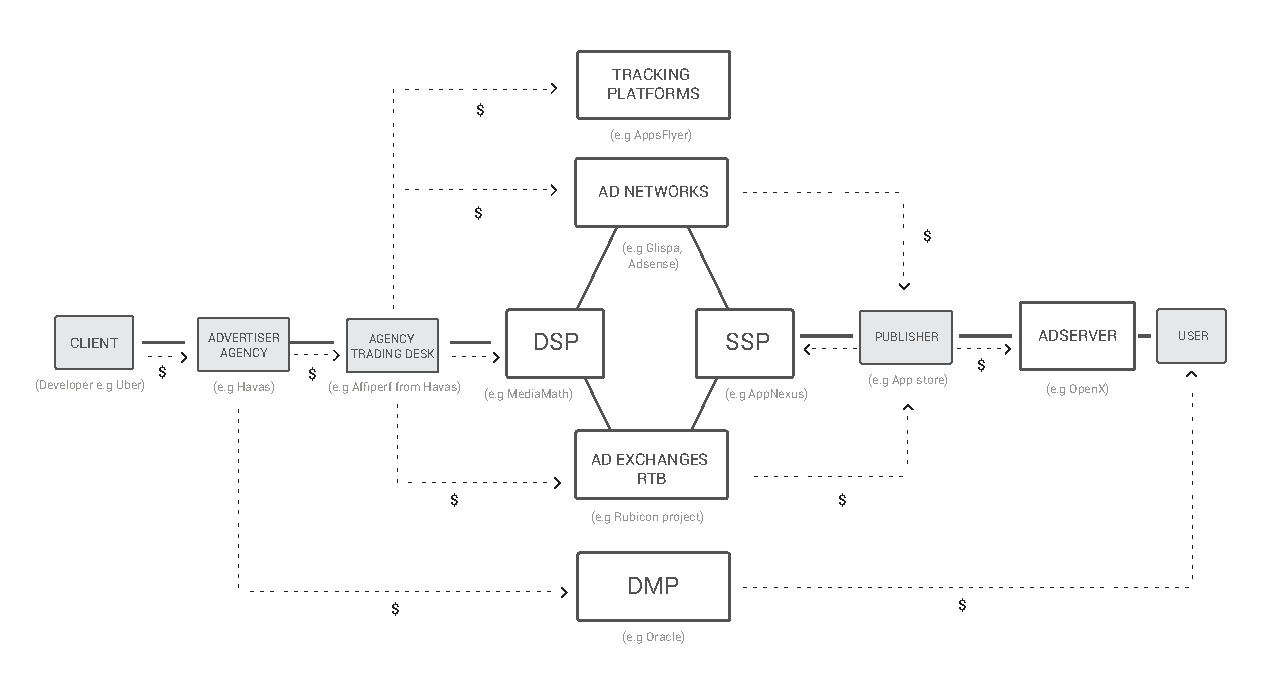
\includegraphics[width=\textwidth]{diagrams/cpi_flow.eps}
\caption{Cost per Installation (CPI) ecosystem.}
\label{fig:cpi}
\end{figure}

For simplicity, we will focus on the Cost per Install (CPI) model shown in Figure \ref{fig:cpi}, since the difference to the other models, like Cost per Action (CPA) or Cost per Thousand Impressions (CPM), is a matter of who shares the risk and captures the value.

In an advertising model where the advertiser (developer) bids for an installation, we have three different moments:

\begin{itemize}
\item {\em Campaign creation}: The developer (advertiser) defines the conditions for the ad to run in the store. Typically, he establishes a value for the bid representing the value that he is willing to pay for an install. There are other types of conditions called ``filters'', which represent target requirements. For example, requirements stating that the campaign must run in a specific country, a specific smartphone, a specific operating system version, and others.
\item {\em Impression}: When the campaign conditions are met and the bid is competitive, the ad is shown. The user may click on the ad to see the complete description of the app.
\item {\em Install}: If the user installs the app, thus converting the impression, an attribution is due and the corresponding money is transferred.
\end{itemize}

% Create a itemize list above 

At each of the above moments, the lack of trust between the developer and the user carries different risks. Table \ref{tab:risks} summarises the different risks at each stage.

% table

\begin{table}[ht]
\centering
\begin{tabular}{|l||l|l|l|} \hline
{\bf Role} & {\bf Campaign} & {\bf Impression}  & {\bf Install} \\ \hline
{\bf User} & & & Is not a real user \\ 
 & & & ({\em R1: Risk of fake person}) \\ 
 & & & Double conversion  \\
 & & & ({\em R2: Risk of double attribution}) \\
 & & & Don't use the app  \\
 & & & ({\em R3: Risk of no attention}) \\  \hline
{\bf Publisher  /}  & & & Selling the data to third-parties \\ 
{\bf App store} & & & ({\em R4: Risk of data leak})\\ \hline
{\bf Developer} & Not enough funds & Run out of & Don't pay \\  
 & to start campaign & budget & the conversion \\  
  & ({\em R5: Risk of default}) & ({\em R5: Risk of default}) & ({\em R6: Risk of repudiation}) \\  
\hline\end{tabular}
\caption{Risks in advertising industry classified by action and by role.}
\label{tab:risks}
\end{table}

The risks presented above are today managed in different ways by the advertising ecosystem and have different impacts:

\begin{tcolorbox}[enhanced jigsaw,sharp corners, drop fuzzy shadow=ShadowColor]

The {\bf\em R1.1: Risk of fake person} consists of the impression of the ad and later installation being presented to a non-real person (bot,...) with the purpose of deluding the advertiser. 


The {\bf\em R1.2: Risk of double attribution} happens with the possibility of the same user to count twice as a conversion, leading the developer to pay two times what was due.


The {\bf\em R1.3: Risk of no attention} consists in the user installing the app that is being advertised but paying no attention to it. Even if they open the app, there is the possibility of no interaction with the app, i.e. the user opens and immediately closes the app. This leads to a zero return-of-investment.


The {\bf\em R1.4: Risk of data leak} consists in the information regarding the user being leaked to third-parties for advertising purposes. Information about the user's preferences are aggregated in Data Management Platforms (DMP) and later used by advertisers in programmatic / RTB targeting. 

The {\bf\em R1.5: Risk of default} consists in the developer creating a campaign but not having enough funds to pay the conversions that are generated in that campaign, leading to him not paying the due amount.


The {\bf\em R1.6: Risk of repudiation} happens when the developer does not recognise the installation, failing to attribute the conversion to the publisher. The attribution is generally monitored by tracking platforms like AppsFlyer, Adjust or Kochava that have multiple variables that can be changed by the developer to define what it considers a real attribution. These variables can take in account the time window period between the click URL and the conversion, the network fingerprint, among others. Attribution, or the lack of it, is harming the industry with only 15\% to 25\% of the real installations being considered conversions\footnote{Values based on Aptoide experience.}.

%XXX what does mining the industry mean?
%XXX provide reference for the 15-25% statement

\end{tcolorbox}

These risks in the Advertising flow will be considered in a section ahead in the design of the AppCoins blockchain.


\subsection{In-App Billing}
\label{subsec:intro_iab}

% Description of In-App Billing inside the stores

In-App Billing (IAB), also called In-App Purchase, consists in the possibility for the user to buy digital items inside an app or a game. Although those items are perceived to be bought inside the App, the items are bought through the app store.

\begin{figure}[!ht]
\centering
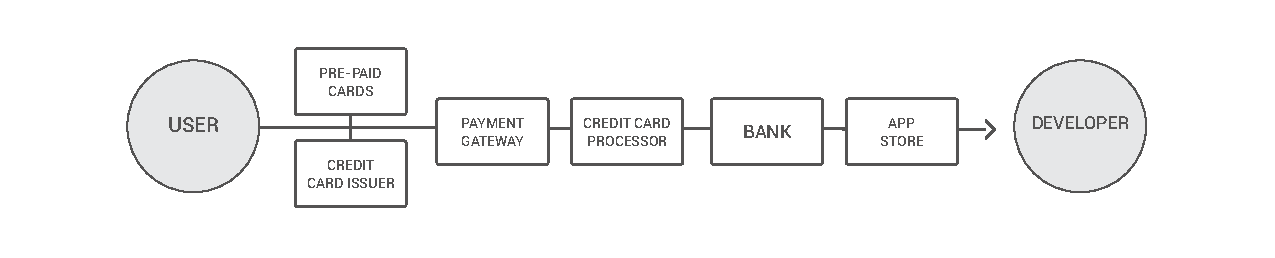
\includegraphics[width=\textwidth]{diagrams/iab_flow.eps}
\caption{Current IAB flow and intermediaries.}
\label{fig:iab_flow}
\end{figure}


The need for the transactions to go through the app store were introduced as mandatory by Apple App Store and then by Google Play. The conditions for the developer's app to be distributed is that all the financial transactions have to be managed by the app store. 

The app store adds some value to this flow: 1) it may know the customer already and have their payment data, thus easing the entrance hurdles for the user and providing a better user experience, 2) it has the trust of the user when the developer may not have it yet and 3) it develops the necessary technology, allowing the developer to focus on the app development.

Although IAB represents a market with a huge volume of transactions processed by Google Play and Apple, there are still two big challenges.

%XXX provide source for "huge volume of transactions by ..."

The number of users with a credit card loaded in the store is still a minority. Only small part of the world population has access to credit card. Alternative methods like pre-paid cards are an approach but they are physical and depend on points of sale, therefore do not scale well.

%XXX provide source for "Only small part of the world population has access to credit card."

On the other hand, some of other payment methods like carrier billing have prohibitive margins that compromise the revenue share of 70\% for the developer. In some markets, the margin of the telecom operator varies between from 35\% to 60\% of the cost of the transaction. The reasons given by the telecom operators are: 1) high risk of fraud that has to be compensated and 2) the users may cannibalise the telecommunications balance so the margin has to pay that possibility.

%XXX provide source for margin being between 35% and 60%

Providing the user has a proper payment method, there are still some risks that have to be mitigated:

\begin{tcolorbox}[enhanced jigsaw,sharp corners, drop fuzzy shadow=ShadowColor]

The {\bf\em R2.1: Risk of user data leak} consists in the information regarding the user being leaked to third-parties for advertising purposes. Information about the user preferences are aggregated in DMP platforms and later used by advertisers in programmatic / RTB targeting.

%XXX R2.1 is copy and paste of R1.4!

The {\bf\em R2.2: Risk of digital goods lost} may happen when a user buys a digital good inside the game or app but it is not delivered. Often, the user does not have a way to recover the payment or claim the digital good.

The {\bf\em R2.3: Risk of double payment} occurs when the user pays twice for the same in-app item purchase. Also in this case, the user may not have a proof that they paid twice.

The {\bf\em R2.4: Risk of digital items cloning} when the user is able to duplicate and transfer the digital good to another user, leading to losses for the developer that charge once for a digital good that is used twice.

\end{tcolorbox}

A platform that handles the IAB transactions has to deal with those risks.


\subsection{App Approval}
\label{subsec:intro_approval}

% Description of today state: central approval, manual QA, automatic QA, time taken, arbitrary approval

\footnote{This section was contributed by Jo\~ao Carneiro, Aptoide backend team member}App approval is one of the more critical challenges of an app store. By definition, the app store is a channel between the developer and the user.

\begin{figure}[!ht]
\centering
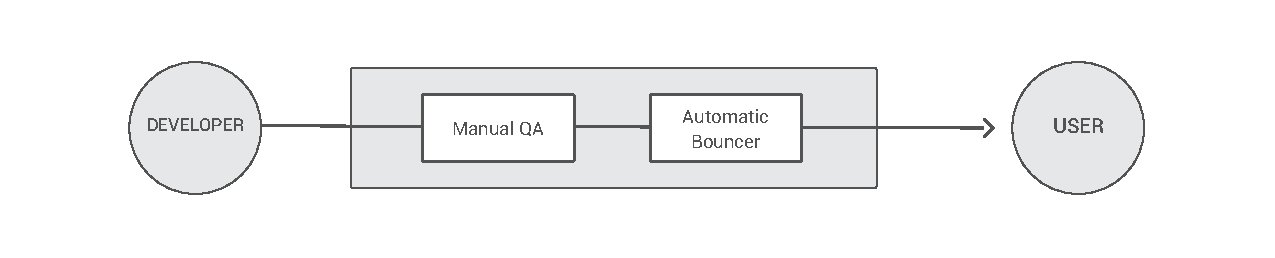
\includegraphics[width=\textwidth]{diagrams/apps_approval_flow.eps}
\caption{App approval in centralised App Stores.}
\label{fig:app_approval_flow}
\end{figure}

% include contribution from João Carneiro
In order to enforce security, legal and business requirements, app stores define limits in terms of acceptable app behaviour and/or content. These policies also mirror the store's philosophy (e.g. defining the acceptable content) and protect both users and developers against unwanted or potentially dangerous behaviour, thus promoting trust. Policies can include general categories such as safety - protecting against malware behaviour, offensive content or physical harm - or legal - protecting privacy and intellectual property. More restrictive stores such as the Apple App Store also imposes strict rules regarding the user interface design, minimum functionality and quality. \cite{GooglePolicyWebsite} \cite{ApplePolicyWebsite}

%XXX I don't get the meaning of "general categories"

The risk of infringement occurs when new apps are added to the store. Therefore, stores which are open to public upload of apps (e.g. Google Play Store or Apple Play Store allow submission by developers) need to ensure that uploaded apps abide by their rules by putting them through a reviewing process. 

The app screening may be performed through manual and/or automatic processes and differ between stores as they are defined by their own policies. The manual process involves a group of people (typically belonging to the Quality Assurance and/or the Security Team) who manually install and test apps on real devices. They examine the apps' behaviour and content in order to decide whether each app respects the store's policy. The automatic process consists of a computer program which automatically analyses the submitted apps and compares features to a given dataset of rules, signatures, unwanted apps, content or behaviour. Multiple techniques may be used by the program to automatically classify given apps into unwanted, accepted or unknown states \cite{Bhattacharya2017}.

Google's Play Store and Apple's App Store, the current largest and most well-known app stores, use a combination of both processes. When a new app is submitted to their store, they first go through an automatic process which will automatically discard identified unwanted apps and then proceed to the manual process. However, the two stores differ in the techniques they use in their automatic processes and the amount of apps that go through manual reviewing \cite{AppleInsiderWebsite, AndroidWhitePaper}.

Apple App Store approval flow is simple. All submitted apps go through an automatic static analysis process, a method which examines the app code without running it. In this process, the apps are analysed for traces of calls to Apple's private API as the company's policy only allows calls to their public API. The identified apps are discarded while all the remaining apps are passed on for manual review \cite{AppleInsiderWebsite, AppleApprovalFortune}. Apple states the following most common reasons for failing their strict manual reviewing process: crashes and bugs, broken links, placeholder content, incomplete information, inaccurate description, misleading users, substandard user interface, advertisements, web clipping, similar apps and not enough lasting value \cite{AppleReviewRejections}. According to Apple, the complete review process takes on average between 24 (50\%) to 48 hours (90\% of submitted apps) \cite{AppleReviewTime}. 

Google's Play Store has a more evolved reviewing system where the automatic process involves a complex machine learning engine. This engine relies on multiple technologies including static and dynamic analysis (where both code and runtime behaviour is analysed), heuristic and similarity analysis (for finding new trends of unwanted apps) and signatures (identifying known unwanted apps). The engine also includes features from external independent security research as well as the developer's behaviour (history with other apps and billing profile) as well as metadata such as ratings and downloads. The automatic process assigns to each application a risk level ranging from safe to harmful. Low risk applications are automatically accepted and high risk applications are automatically rejected. Apps with medium risk level are submitted for manual review \cite{AndroidWhitePaper}. 

\medskip

Although these app approval systems are capable of detecting a large number of unwanted apps, they also pose problems to developers. Apple's automatic process has shown problems with false positives and rejecting legitimate apps \cite{AppleInsiderWebsite} and their strict policy is known to frequently change the categories of rejected apps, posing problems to developers of such apps. Also, Apple's reviewing process strongly based on human analysis is known to have flaws, namely not being able to detect apps which hide their malware behaviour by being inactive for a given amount of time and showing a regular behaviour in order to escape the human test \cite{AppleFlaws1}. Other reports \cite{AppleFlaws2} have also shown a big presence of scamware in Apple's store where apps are able to scam users into paying for unneeded services. Google's more automated system has also been shown to have flaws \cite{AppleApprovalFortune} due to its more permissive system with apps being accepted without manual evaluation. Frequent security reports show breaches in the security control of Play Store reporting the existence of multiple malware (ransomware, backdoor and trojans) infected apps compromising several millions of devices and thus posing serious threats to users \cite{GoogleMalware1, GoogleMalware2, GoogleMalware3}.

Both Apple's App Store and Google's Play Store have a history of refusing and banning apps. Examples of recent complaints include the rejection of the social network GAB's app by both Apple and Google \cite{AppRefusedGAB}, the refusal of music streaming service Spotify's app update \cite{AppleRefuseSpotify} or the Anti-Spam App \cite{AppleRefuseTRIAD} by Apple and the rejection of Popcorn Time, TubeMate, Adguard or Fildo by Google \cite{GoogleBannedApps}. However, these rejections are often considered unfair by developers who claim an abusive and anticompetitive behaviour as the apps conflict with other services provided by the app stores and have motivated a number of complaints to legal authorities \cite{AntiCompetitiveClaim}. \\

As described above, several risks can be found from the current centralised app approval processes:

\begin{tcolorbox}[enhanced jigsaw,sharp corners, drop fuzzy shadow=ShadowColor]

The {\bf\em R3.1: Risk of Malware} is the possibility of an app or game submitted to the app store being infected with a virus or malware that steals data or damages the user's device.

The {\bf\em R3.2: Risk of user data leak} consists in the information regarding the user being leaked to third-parties for advertising purposes. Information about the user's preferences are aggregated in DMP platforms and later used by advertisers in programmatic / RTB targeting.

%XXX again, R3.2 is just a copy and paste of R1.4

The {\bf\em R3.3: Risk of censorship} when an app store blocks the publishing of an app or game based on political, religious or social factors that are subjective and totally unrelated with technical aspects. The censorship can be self-inflicted when the company running the app store follows orders or guidelines of national governments or can be result of technical external restrictions that limits the access to the app store (The Great Firewall of China, for example).

The {\bf\em R3.4: Risk of arbitrary decisions} happens when the app store denies the distribution of an app based on ``anti-competition clauses'' \cite{PlayTermsService} or other reasons only related to its business interest, even if the interest is in other markets or industries.

\end{tcolorbox}

\subsection{Paper organisation}

This paper is organised in the following chapters. In this chapter we started to introduce the flows, the current challenges and the flaws they carry.

Chapter \ref{sec:design} will propose the overall design of the solution for the core app store flows supported by blockchain technology. 

Chapter \ref{sec:protocol} will dive deep in the blockchain technology, presenting the main data structures and algorithms that are proposed.

The current limitations of the blockchain technology when applied to app stores are introduced in Chapter \ref{sec:limitations}.

In Chapter \ref{sec:related}, related work that shares common approaches with the AppCoins protocol are introduced, as well as projects that inspired parts of the AppCoins protocol.

% TODO replacing 6 by the \ref tag

The future protocol developments will be included in Chapter 6 and this document will end with acknowledging the contributions of the several community members that contributed to this document with their suggestions and opinion.




\section{Design of the Solution}

\label{sec:design}
%missing introduction?

\subsection{Assumptions}

% A table 

Building a model always depends on assuming certain assumptions. The generalisations taken in the 
assumptions allows one to focus on the global mechanics and do not take corner cases into account. 
As exceptions, they are part of the reality but they do not have material importance to change the result 
of the model.

The design of the AppCoins platform was made having the following eight assumptions:

\begin{itemize}
\item {\bf\em A1 Crowdsourcing}: Community wisdom works for big numbers better than individual 
wisdom \cite{Surowiecki:2005:WC:1095645};
\item {\bf\em A2 Incentives}: If there are enough incentives, community contributes;
\item {\bf\em A3 New}: A new developer is always an unknown developer;
\item {\bf\em A4 Trusted:} The Apps from a Trusted Developer are Trusted Apps;
%chose between how to use capitals: Developer vs developer in A3 and A4
\item {\bf\em A5 Dispute}: - In a dispute, if 50\% + 1 of the community is honest, the right side wins;
\item {\bf\em A6 Reputation}: - Transactions registered in the blockchain ledger (IAB, Ads) reflects well 
the trustworthiness and reputation of a developer;
\item {\bf\em A7 Unknown downloads}: - If the app downloads made by the users come from more than 
5\% of unknown developers, users will start to have trust in unknown developers.
\item {\bf\em A8 Zero-day}: - A community dispute may take 30 days. While the dispute is handled, the 
app stores have the option to hide the app to avoid zero-day attacks.
\end{itemize}



\subsection{Client side support}

Besides the blockchain technology, the environment where the user is running the app store should 
also support the AppCoins protocol.

% TODO }: include quote
%missing context and connection to previous sentence?

As Android represents 86\% of the smartphones market, we focus an implementation analysis in that 
platform. However, many of the constraints and solutions are applicable to other smartphone operating systems.

This subsection\footnote{This section was contributed by Marcelo Benites, Aptoide Android team 
member} aims to describe a client-side method, running in the smartphone's untrusted environment, to 
register that a user is paying attention to an app (installed from an app store) for a certain amount of time. Once those requirements are met, a \textit{proof-of-attention} (\textsf{PoA}) is requested and stored in the 
blockchain.
 
%XXX describe what is a proof-of-attention
 
Concepts definition: %improve this introductory sentence?
\begin{itemize}
\item {\bf App store}: PoA compliant app store Android app.
\item {\bf Application}: Android app installed from the app store.
\item {\bf User}: user registered in the app store.
\end{itemize}

When designing a solution, two main factors should be taken into account: reliability and availability. 
Reliability consists in avoiding fraud. Once a \textsf{PoA} is generated, it has to have a high level of 
confidence that a user paid attention to an app installed from an app store. Availability consists in 
making sure that whenever a user pays attention to an app installed from an app store, the app store 
will be aware of that and will request the \textsf{PoA} once the requirements are met. %requirements?

The app store process has to be running when the user is paying attention to an app in order to request  
the \textsf{PoA}. Latest releases of the Android operating system (Android OS) - from Lollipop (API 
level 21) onwards - have been limiting the ability of app processes to run while the app is in the 
background. In our scenario the app store process could eventually be killed by the Android OS while 
not being in the foreground. In order to overcome that issue, we will take advantage of the Binder 
framework to bind the app and app store's processes while the app is in the foreground, which will 
ensure that the app store process is not killed by the Android OS. 

\begin{figure}[!ht]
\centering
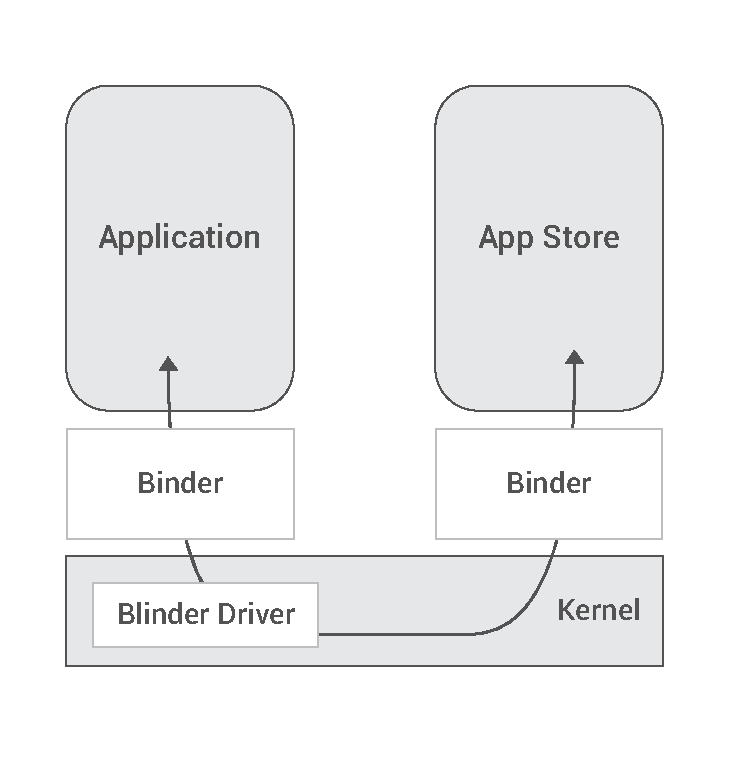
\includegraphics[width=0.5\textwidth]{diagrams/binder_diagram.eps}
\caption{Operating system binder.}
\label{fig:binder}
\end{figure}

Binder framework is a core component in Android architecture and its main goal is to simplify Inter-
Process Communication (IPC). Binder is implicitly used whenever an app communicates with OS 
services or with other apps through the Android Java API Framework. The Binder framework will also 
provide information regarding the app process, which will positively contribute to the app store 
\textsf{PoA} reliability.

Once the app and the app store's processes are bound, the app store will periodically verify whether 
the app is in the foreground and the user is actively interacting with the device. In order to certify that 
the user is paying attention to the app, the following conditions should be met:
%are conditions the same as what was previously called requirements?

\begin{itemize}
\item The app's process must be bound to the app store's process.
\item The app must be in foreground.
\item The device screen must be on.
\item The device must not be locked. 
\item The signature of the app must be verified on the app store's servers.
\end{itemize}

To assure that the app's process is bound to app store, Binder and PackageManager APIs can be used. 
To verify whether an app process is in the foreground, both ActivityManager, UserStatsManager and 
%or?
 PackageManager APIs can be used. To check whether the device screen is on, the PowerManager 
and Display APIs can be used. Regarding the state of the lock screen, the KeyguardManager API can 
be used. 

Every application has to be signed by the developer before being installed on an Android device. App 
stores have access to the apps' signatures and can validate by confirming whether they match with the 
signature on their servers. If the signature does not match, the app may have been tampered with. To obtain the app's signature, the Binder and PackageManager APIs can be used.

\subsubsection{Limitations client-side}

The proposed solution has some limitations regarding reliability - imposed by Android's inherently 
insecure environment - and Android API availability - due to Android's version fragmentation and app 
store permission level. The use of several different Android APIs can help harden the solution 
against an attacker but can not assure full protection against fraud on the client side. In order to 
mitigate fraud, a system has to have different security layers both on the client side and the server side. 

In Android some APIs are considered sensitive and require system-level permissions to access them. 
Usually system-level can only be granted to system applications (pre-installed on the device by 
manufacturers). Also some APIs are only available in certain versions of Android. Table \ref{table: permissions} summarises the APIs needed to generate the \textsf{PoA} and their availability:

\begin{table}[H]
\scriptsize
\centering
\begin{tabular}{|l|l|l|l|l|l|}
\hline
\textbf{API Class}                          & \textbf{API Method}                  & \textbf{Min API}      & \textbf{Max API}       & \textbf{Permission Level}               & \textbf{Permission}                             \\ \hline
\multirow{2}{*}{PowerManager}      & isScreenOn                  & API 7       & API 19       & \multirow{2}{*}{None}          & \multirow{2}{*}{None}                  \\ \cline{2-4}
                                   & isInteractive               & API 20      & None                  &                                &                                        \\ \hline
Display                            & getState                    & API 20      & None                  & None                           & None                                   \\ \hline
Binder                             & getCallingUid               & API 1      & None                  & None                           & None                                   \\ \hline
\multirow{2}{*}{ActivityManager}   & getRunningAppProcesses      & API 3      & API 21     & None                           & None                                   \\ \cline{2-6}
                                   & getRunningTasks             & API 1      & API 20       & Normal-Level                   & GET\_TASKS                             \\ \hline
\multirow{2}{*}{PackageManager}    & getPackagesForUid           & API 1      & \multirow{2}{*}{None} & \multirow{2}{*}{None}          & \multirow{2}{*}{None}                  \\ \cline{2-3}
                                   & getPackageInfo              & API 1      &                       &                                &                                        \\ \hline
\multirow{2}{*}{KeyguardManager}   & isKeyguardLocked            & API 16  & \multirow{2}{*}{None} & \multirow{2}{*}{None}          & \multirow{2}{*}{None}                  \\ \cline{2-3}
                                   & isDeviceLocked              & API 23 &                       &                                &                                        \\ \hline
\multirow{2}{*}{UsageStatsManager} & isAppInactive               & API 23 & None                  & \multirow{2}{*}{System-Level} & \multirow{2}{*}{PACKAGE\_USAGE\_STATS} \\ \cline{2-4}
                                   & queryAndAggregateUsageStats & API 21    & None                  &                                &                                        \\ \hline
\end{tabular}
\caption{\textsf{PoA} generation Android APIs. The \textit{UsageStatsManager} requires a System-Level permission but the PACKAGE\_USAGE\_STATS can also be obtained by a normal application if the user explicitly enables it in the Settings.}
\label{table: permissions}
\end{table}

We can only have an implementation that fulfils all the requirements to certify that the user is paying 
attention to the app with a minimum Android version of Jelly Bean (API 16) and above. The Android 
version limitation is not relevant since according to Google statistics, only 1.2\% of the Android devices are not running version Jelly Bean (API 16) or above. %reference missing

Also, UsageStatsManager is necessary from Lollipop (API 21) onwards requiring that, either the app 
store app is a system app, or asking the user to explicitly go to Settings and give the permission. Since 
in the App Economy the user will be rewarded by the attention given to apps, it will be easy to convince 
him to manually provide the permission in the case where the app store is not a system application.


\subsection{Protocol Overview and sketch}


The AppCoins protocol is depicted in Figure \ref{fig:design}. It consists in 3 main blocks: Advertising, 
Developer's Reputation (Rank) and IAB.

\begin{figure}[!ht]
\centering
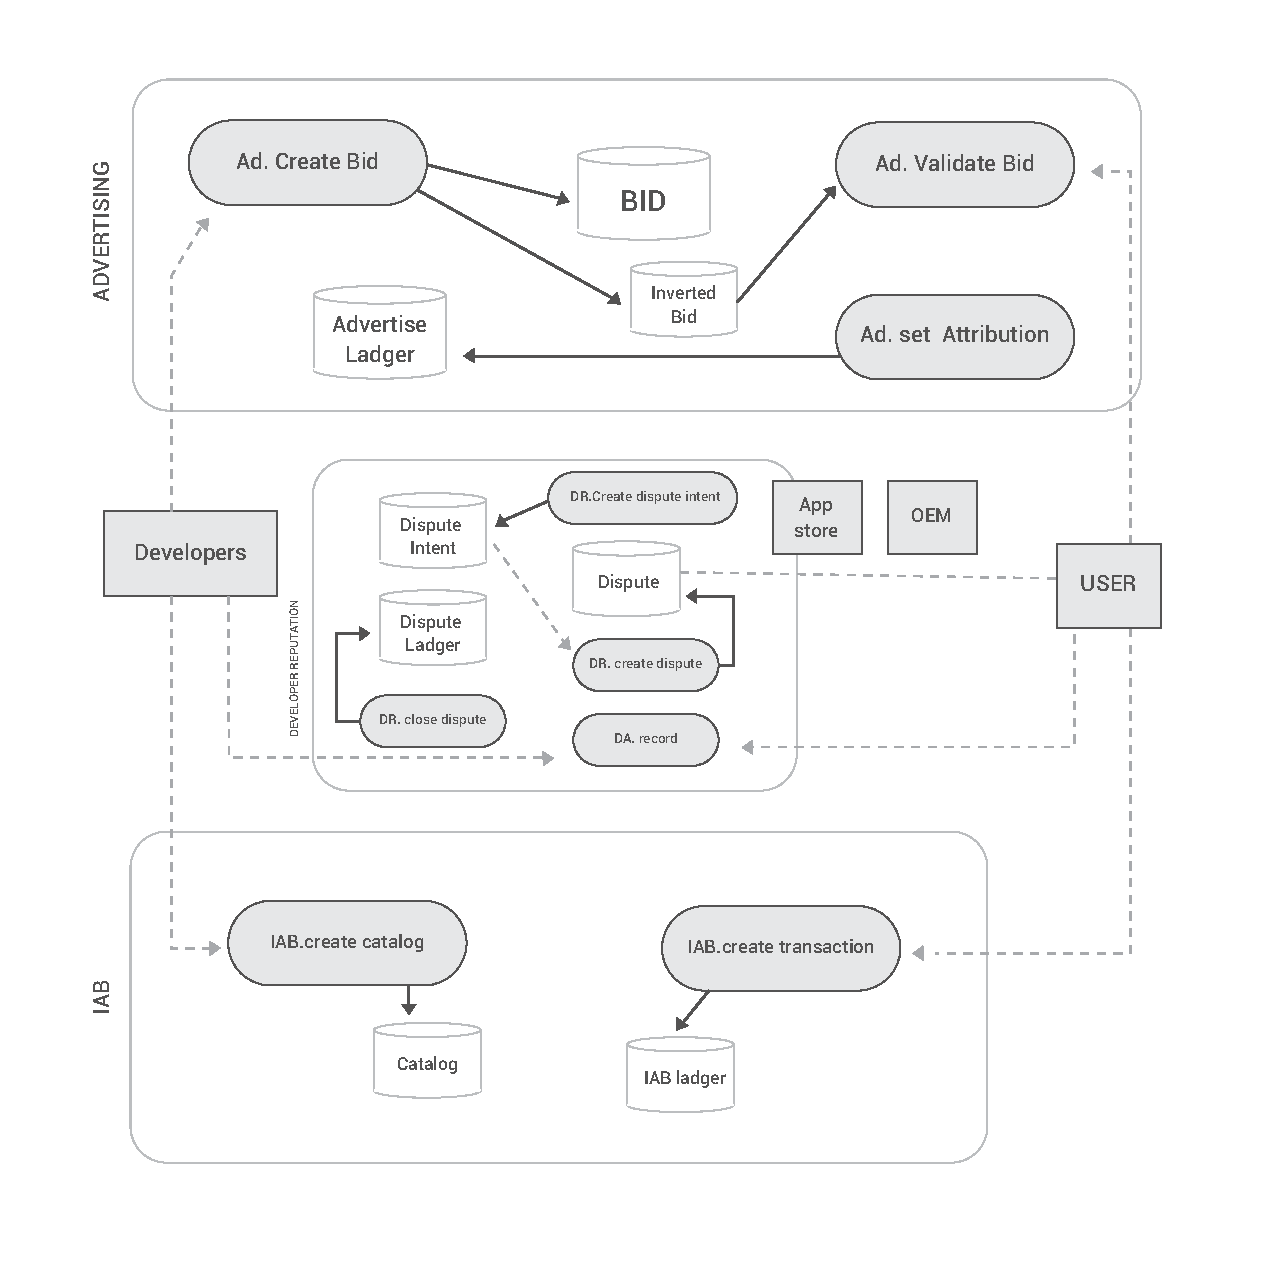
\includegraphics[width=0.8\textwidth]{diagrams/design.eps}
\caption{Overall design of AppCoins and blockchain interactions.}
\label{fig:design}
\end{figure}

Inside each block we see the interactions between the ecosystem players and the blockchain. The 
rounded squares represent functions / methods of smart contracts that implement business logic. The 
cylinders represent data stored in smart contracts' own storage or event logs. \\

{\bf Advertising}

The protocol was defined such that most risks in Section \ref{subsec:intro_ads} are avoided or at least mitigated. By leveraging blockchain technology and its requirements of transparency, accountability and verifiability of processes, we avoid creating a middlemen-dependent economy and add value both for the advertisers/developers and the users. \\

As explained in Section \ref{sec: introduction}, there are three moments in an advertising model: campaign creation, impression and attribution (which can be an installation, opening of the app, etc).  In AppCoins protocol, an attribution does not happen when the user installs the app or game, but after the app is opened for 2 minutes. This poses the problem of how can the app store prove that a user did indeed open the app and had it opened for the required period of time. Our protocol introduces a \textit{proof-of-attention} \textsf{PoA}, which allows the developers to verify that users did actually paid attention to the app for the required time. \\

Since the smartphone is an untrusted environment, there is not a total guarantee that the user is real or that the app store stub installed in the phone was not tampered. However, identity is checked server side by the app store using network fingerprint (IP, routing information, etc) as it is done today by the tracking platforms. Similar challenges to \textsf{PoA} are addressed in BAT \cite{BAT}. \\

From the requirement of privacy, the protocol itself does not expose any user information at any time and interaction with app stores. The only information that can be seen by others are the wallet addresses when a transaction occurs. Concerning risk \textsf{R1.4}, since the addresses are not linked to any sensitive user information (e.g. email), there is no leakage of user data. \\

Regarding risk \textsf{R1.6}, developers can claim that a certain user did not actually do the required action to be given the attribution, i.e. that either the app store, the user or both are being dishonest. By providing a \textsf{PoA} and storing the transactions in the blockchain, they become verifiable by anyone, including the developer. Since the developer can verify the proof, it becomes clear that the protocol avoids the risk of repudiation. \\

Since our solution proposes that no middlemen is needed within the advertising model, there is the need to have the protocol being able to enforce the payments between the developer and the other parties, which are the user, the app store and the OEM. The only way to make sure the entirety of the funds that the developer wants to put available for the campaign exist is to lock them in a different wallet, which is where the smart contract for the campaign will be running. Since they are locked, the developer cannot spend them before the campaign is over and there is no possibility for the developer to be in default. In addition, when there is an impression, the amount of tokens to be paid for that conversion need to be locked as well. This serves to avoid race conditions, which can occur when the funds still available in the campaign are for $X$ attributions but $Y$ users are getting impressions for the campaign (with $X < Y$). If this would be possible, some of the $X$ users would install the app but when they opened it and paid attention to it for the required time, thus being eligible for the attribution, they would not get the attributed because there would be no more funds available. This means that different wallets need to exist that serve to lock funds for the already made impressions. If the attribution for a certain impression does not occur after some designated amount of time, then the funds would be unlocked and placed back in the campaign wallet. This funds captivation scheme is exemplified in Figure \ref{fig:wallet_cpi_flow} and avoids the risk \textsf{R1.5}.\\

{\bf IAB}

The IAB use case has the risks outlined in Section \ref{subsec:intro_iab}, which the protocol needs to either avoid or mitigate. \\

As in the Advertising use case, since the protocol follows the requirements of blockchain technology, and in particular the requirement of privacy, the protocol only exposes wallet addresses when transactions occur. These need to be publicly available in order to have the possibility of verifying transactions but do not carry any link to personal user information (for example, the email of the user). Therefore, risk \textsf{R2.1} is partially avoided. \\

The protocol is built to allow for transparency between users, developers and app stores. Transparency means that transactions between parties are public and verifiable, but only regarding token exchange. This means that the protocol is not intended to store items or any other form of goods/value. This tracking, as it is today, is to be done directly by users and developers, i.e. when the user pays for an in-app item, it is the user's responsibility to check if the item is transferred or not. The store, retrieve, and exchange of digital items between users is out of the scope of the AppCoins solution. Nonetheless, having the transactions publicly available mitigates this problem, which is referred to as risk \textsf{R2.2}, but does not completely avoid it. However, because of having the transactions publicly available, the protocol avoids risk \textsf{R2.3} because the user only sends more tokens in exchange for an in-app item if wanted. \\

Regarding item cloning, as it has been said, the protocol itself does not deal with in-app items or their exchange, only with the token transfers in the scope of in-app purchases. Hence, there is no possibility within the protocol to clone items and neither to send them to other users. Therefore, risk \textsf{R2.4} is not addressed by the protocol at this version.\\


{\bf Developer Reputation}

This use case is the one that may dictate if a developer is trustable or not. Therefore, if the protocol defines ways to mitigate and avoid malware attacks across the app stores operating within the protocol, then the adoption of the protocol by app stores can be greatly increased. \\

As it was said in Section \ref{subsec:intro_approval}, the malware scanning process is different for all the app stores, as are the reasons for blacklisting apps. An app store that is not showing an app to its users because it is from a competitor or for censorship purposes, although the app was considered ``trusted'' in the blockchain, is then exposed in the community. If the malware knowledge is not shared across app stores - the current state - will fin act harm users because one app with malware may have already been blacklisted in an app store but it still available on others. Our protocol deals with this problem by attributing a reputation level to the developers, which is then extended to all their apps. \\

The reputation of a developer has two components: the rank and the rank level. The rank can have the values of \textit{"Unknown"}, \textit{"Trusted"} or \textit{"Critical"} and it states if a developer is new to the community, if it is already known and considered honest or if it is considered dishonest, respectively. The rank level is represented by an integer starting at 1 and does not have a maximum level for the \textit{"Trusted"} rank. However, for the other ranks it is fixed at 1. This derives from the fact that when a developer is \textit{"Unknown"}, it is just because the developer is new in the network and the goal is that the developer leaves the rank to become \textit{"Trusted"}. On the other hand, being a \textit{"Critical"} developer means the developer is dishonest and we do not intent to have different levels of dishonesty in the network. Figure \ref{fig:approval_state_diagram} shows the different ranks a developer can have and how to move from one rank to another. \\

\begin{figure}[!ht]
\centering
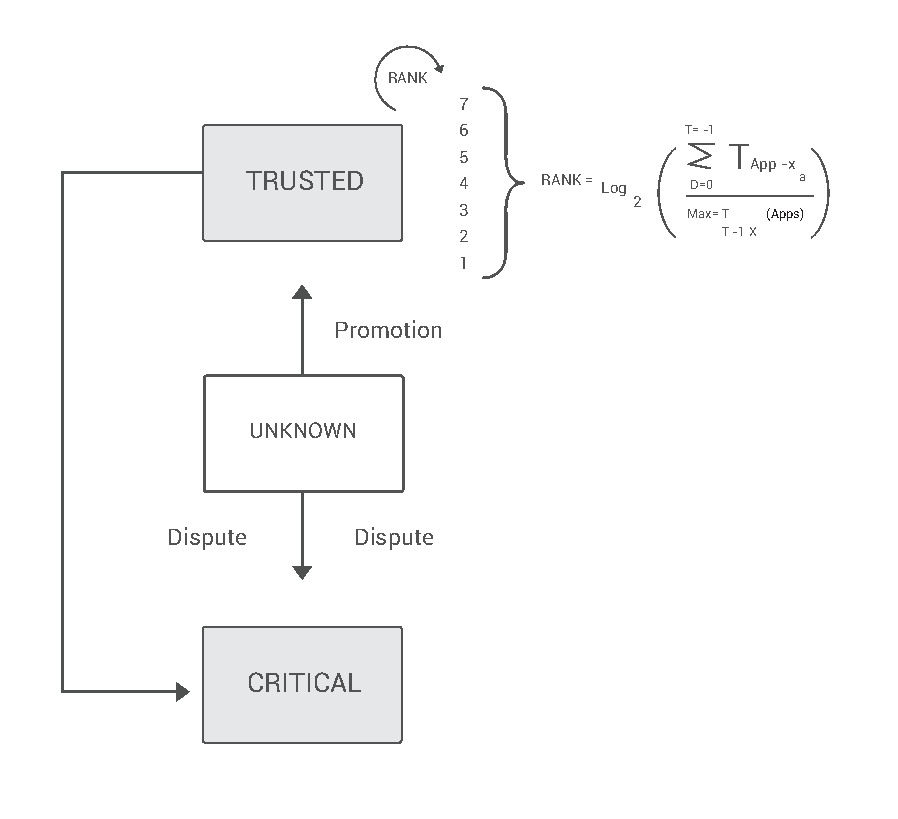
\includegraphics[width=0.5\textwidth]{diagrams/approval_state_diagram.eps}
\caption{Approval state changes.}
\label{fig:approval_state_diagram}
\end{figure}

As it can be seen, there are two processes by which the rank can change: \textit{promotion} and \textit{dispute}. A \textit{promotion} is an automated process which takes into account the number of transactions occurred in the developer's apps and compares them to the transactions of other popular apps from trusted developers. If the developer's apps compare well against others (this comparison is detailed in Section \ref{subsec:protocol_devrank}), the rank is either increased to \textit{"Trusted"} or the rank level goes up one level in the case where the developer is already \textit{"Trusted"}. \\

Regarding the \textit{dispute}, it is a mechanism to punish developers that deliver bad apps, either because they contain malware or they are fake, i.e. do not do anything and may contain only ads. This process of judging developers has been a centralised process in app stores and our protocol introduces a way to have it done by the community, since it is the community that uses the apps. The protocol provides a way to open a dispute against a developer, i.e. any user can claim that a developer is dishonest. When a dispute is started, which at this point we call as a \textit{dispute intent}, any user can answer it within the next 7 days. The user answering it, which would mean that the user is claiming the developer is honest, can be any user and does not need to be the developer. If the dispute intent is answered, a dispute is opened and stays open for 30 days. Within this time period, any user can join any side of the dispute, either the \textit{Contestants} - users who claim that the developer is dishonest - or the \textit{Pleaders} - users who claim the developer is in fact honest. If the dispute intent is not answered by anyone, the dispute intent is closed without opening a dispute and the developer's rank changes to \textit{"Critical"} along with the rank of all the apps of that developer. \\

In order to join a dispute, a user needs to put an amount of tokens into stake. The amount of tokens is chosen by the user and express the confidence in the side the user is joining. When the 30 days of the dispute are over, the side which collected the biggest amount of tokens wins. The winning side gets a refund of the tokens pledged plus 10\% of the pledge of the losing side. This 10\% is divided according to the percentage each user had pledged within the winning side pledge. The losing side gets a refund, where the pledge of each user has a cut of 10\%. Regarding the change in the developer's rank, if the \textit{Contestants} win, the developer's rank changes to \textit{"Critical"} and all the apps of the developer also have their rank changed. On the other hand, if the \textit{Pleaders} win, the developer's rank remains unchanged. \\

The dispute mechanism transfers power back to the community, which can also include the app stores. Since it is the community deciding whether a developer and the corresponding apps are to trusted or not, the developers reputation and the reasons for it are public to everyone. If there is a change in the reputation of a developer, the community knows when it happened and knows it was a decision made by them, instead of being obscurely made by one app store. This mitigates the risks \textsf{R3.3} and \textsf{R3.4}. \\

Risk \textsf{R3.2} is similar to risks \textsf{R1.4} and \textsf{R2.1} and the reason why it is avoided by the protocol is the same.


% a diagram that integrates all the players
% the circular but more geek 

%(Include a diagram with the players - component diagram 

% Could be a sequence diagram as in Filecoin diagram 

% (In-App Billing, Advertising, Reputation builder) 

%




\section{AppCoins: Protocol Construction}

Our solution solves the use cases of Advertising, In-App Billing (IAB) and Developer Reputation within App Stores by leveraging the blockchain construction to create value for the different participants.\\

As it works today, advertising in App Stores is a flow composed by a campaign created by the developer, which is submitted to the several networks of campaigns. App Stores then connect to these networks and get the active campaigns, trying to have their users converting them. As it is now, the value is diluted through all the networks and the most relevant players, which are the developers and the App Stores, are the ones losing the most value, since the latter receive a small amount per conversion compared to the networks, and the former have to pay more than necessary in order to make it interesting for the App Stores to get their campaigns.

The developers and the App Stores should be the players getting the most for their effort, since they are the creators of most of the value in the flow by either creating the apps or by distributing and making them available for the users.\\

In IAB, developers provide content inside their apps, which can be exchanged for money. They integrate third-party SDKs that handle the payments and those third-parties (e.g. Google Play) receive a large amount of the payments, which is between 15\% to 30\% for the larger players in the market (Google Play \footnote{https://support.google.com/googleplay/android-developer/answer/1153481}, Apple \footnote{https://developer.apple.com/app-store/subscriptions/}).

Once again, the players creating the most value, i.e. the developers, should be the ones actively rewarded for their effort and the players supporting them should, i.e. App Stores, not ask for so much in return.\\

Moreover, in both the above scenarios, the OEMs that preload the App Stores in their devices are not included in the value chain of all these transactions. Our solution comprises incentives for OEMs to preload App Stores that add the most value to users as well as to them.\\

The Developer Reputation problem is the one from the mentioned three that, when not addressed properly, can harm users the most. Malignant apps can harm users in several ways, ranging from the most extreme as theft of personal information and device inoperability, to the less harmful as apps containing (almost) only ads or non-working apps. For App Stores with already considerable reach, i.e. already with several millions of users, malignant apps can find their way to a significant amount of devices and thus need to be taken care of before reaching the users.

Today this assessment of apps and developers is done in a centralised way, i.e. each App Store uses its own system, and there is no shared knowledge between App Stores. Our solution includes an approach for the categorisation of developers based on the usage of their apps by the users, and the ability to share knowledge between App Stores.\\

In this section, we present the data structures and algorithms used to solve each of the aforementioned use cases. It will be organised as follows: a section for each use case and subsections explaining the data structures and the algorithms.

\subsection{Advertising}

Advertising campaigns in the context of a blockchain construction must be constructed in a way to overcome the following problems:
\begin{itemize}
\item \textit{Double attribution problem}: For all instances of the same bid (explained in \ref{sssec:ads_ds}) in different App Stores, a user can only be attributed once.
\item \textit{Bid refutation}: A developer must not be able to state that he did not create a bid if it is not true.
\item \textit{Bid validation}: A developer must be able to confirm that the attribution rules match the ones submitted at campaign (explained in \ref{sssec:ads_ds}) creation time.
\end{itemize}

\subsubsection{Data Structures} \label{sssec:ads_ds}

\noindent \textbf{Campaign}. A \textit{campaign} is a statement of intent to pay the attention of users. Developers create \textit{campaigns} and submit them to App Stores, which in turn match and propagate them to users. Campaigns are composed by an amount of funds, a duration, the amount of tokens per attribution, and the filters (app name, app version, geolocation,...). Please refer to Table \ref{table: data_structures_ad} for more details. \\

\noindent \textbf{Bid}. A \textit{bid} is a mapping between developers and the users in an App Store that match specific campaigns created by developers. It also contains the funds available for the \textit{bid} and the amount of tokens per attribution, and its duration.\\

\noindent \textbf{Inverted bid}. An \textit{inverted bid} is a mapping between users and the bids they are participating in for a specific app store. See Table \ref{table: data_structures_ad} for more details.\\

\noindent \textbf{Advertising Ledger}. The \textit{advertising ledger} is the record of attributions, i.e. users that did the required action (having an app open for at least 2 minutes) for a bid. The ledger is populated in a way that avoids the \textit{double attribution problem}, i.e. bids in different App Stores for the same apps in similar time intervals need to be identifiable across all the stores, as well as the users.

\begin{table}[H]
\footnotesize
\centering
\begin{tabular}{|p{.5\textwidth}p{.5\textwidth}|}
\hline
\multicolumn{2}{|c|}{Data Structures} \\
\hline \vspace{0.05cm}
\textbf{Campaign} & \vspace{0.05cm} \textbf{Bid} \\
campaign $C_{ij} := \langle F_{ij}, \Delta t_{ij}, T_{ij}, filters \rangle_{D_{i}, AP_{j}}$
\begin{itemize}
	\item Funds $F_{ij}$, the amount of tokens the developer $D_{i}$ is willing to spend for $C_{ij}$ in an app store $AP_{j}$
	\item Duration $\Delta t_{ij}$, the duration of $C_{ij}$ in $AP_{j}$
	\item Tokens per attribution $T_{ij}$, the amount of tokens to be sent from $D_{i}$ and distributed to the other parties per attribution
	\item Filters, the specifics of $C_{ij}$, as the app name, app version, geolocation of $C_{ij}$, and others available to $D_{i}$
\end{itemize}
& bid $B_i : \{D_1 \to (U_1..U_n)\}_{AP_j}$
\begin{itemize}
	\item Developer $D_i$, developer that submitted a bid $B_i$ to the app store $AP_j$ 
	\item User $U_i$, user matching the filters of campaign $C_{ij}$ associated with bid $B_i$ in app store $AP_j$
\end{itemize} \\
\textbf{Inverted Bid} & \textbf{Advertising Ledger} \\
inverted bid $IB_i : \{U_1 \to (B_1..B_n), U_2..\}_{AP_j}$
\begin{itemize}
	\item User $U_i$, user matching one or more bids $B_{i..n}$ in app store $AP_j$
	\item Bid $B_i$, bids submitted to app store $AP_j$
\end{itemize}
& advertising ledger $L_{Ad} : (A^{1}_{t}..A^{n}_{t})$
\begin{itemize}
	\item Attribution $A^{i}_{t}$, $i$-th attribution in the advertising ledger $L$, which is composed as a mapping $A^{i}_{t} : \{B_{N}^{j} \to (U_{N}^{1}..U{N}^{n})\}$, where $B_{N}^{j}$ is the standardised bid $B_j$ across all the app stores where it is defined and $U_{N}^{i}$ is the normalised user $U_i$ across all the app stores
\end{itemize} \\
\hline
\end{tabular}
\caption{Data Structures for Advertising Use Case}
\label{table: data_structures_ad}
\end{table}

\subsubsection{Algorithm construction}

Table \ref{table: ads_use_case} presents in pseudo-code a more in-depth definition of the following methods. \\

\noindent \textbf{Create bid}. When a campaign is submitted to the App Store, the \textsf{CreateBid} method creates the associated bid $B$ containing the mapping $M$ between the developer $D$ and the set of users $U$ of the app store that match the filters. The inverted bids $IB_{i...n}$ of the app store containing the mapping between users and the bids they are in are created or updated, if they already exist. In addition, the funds $F$ the developer wishes to allocate to the campaign are sent from the developer's wallet $W_D$ to the bid's contract wallet $W_B$. Since the created bid is in the blockchain accessible to every user, it is used to overcome the \textit{bid refutation} problem.\\

\textsf{AD.CreateBid}
\begin{itemize}
	\item INPUTS:
	\begin{itemize}
		\item Campaign parameters:
		\begin{itemize}
			\item Funds $F$
			\item Duration $\Delta t$
			\item Tokens paid per attribution $T$
			\item Filters (geolocation, app name, app version,...)
		\end{itemize}
		\item Developer $D$
		\item App Store $AS$
	\end{itemize}
	\item OUTPUTS: Bid $B$ and inverted bid $IB$
\end{itemize}

\noindent \textbf{Validate bid}. When a bid is to be shown to the user $u$, \textsf{ValidateBid} validates that bid in the blockchain to confirm if it is a valid bid and if the user $u$ matches its filters. In order to avoid the scenario where there are not enough funds available in the bid for the user, the tokens per attribution $T$ defined in the bid are sent to the bid's captivation wallet $W_C$ for a period of time. The method is used to overcome the problem of \textit{bid validation}. \\

\textsf{AD.ValidateBid}
\begin{itemize}
	\item INPUTS:
	\begin{itemize}
		\item User $u$
		\item App Store $AS$
	\end{itemize}
	\item OUTPUTS: Result $R$ (0 or 1)
\end{itemize}

\noindent \textsf{Set attribution}. When a user has been attributed to a bid $B$, i.e. the user performed the required action (e.g. had the app open for at least 2 minutes), \textsf{SetAttribution} checks the advertising ledger $L_{Ad}$ to make sure the user $u$ has not yet been attributed to the bid $B$ and if so, the attribution is written in the ledger and each participant receives the correspondent tokens, i.e. the user, OEM and app store receive $T_u$, $T_{OEM}$ and $T_{AS}$, respectively. Since the method is constructed in a way such that the same user is unable to be attributed the same bid in different app stores, it avoids the \textit{double attribution problem}. \\

\textbf{AD.SetAttribution}
\begin{itemize}
	\item INPUTS:
	\begin{itemize}
		\item User $u$
		\item Bid $B$
	\end{itemize}
	\item OUTPUTS: Result $R$ (0 or 1)
\end{itemize}

\begin{table}[H]
\scriptsize
\centering
\begin{tabular}{|p{.5\textwidth}p{.5\textwidth}|}
\hline
\multicolumn{2}{|c|}{Advertising Use Case} \\
\hline \vspace{0.1cm}
\textsf{AD.CreateBid}
\begin{itemize}
	\vspace{-0.3cm}
	\item INPUTS:
	\vspace{-0.4cm}
	\begin{itemize}
		\item Campaign parameters:
		\begin{itemize}
			\item Funds $F$
			\item Duration $\Delta t$
			\item Tokens paid per attribution $T$
			\item Filters (geolocation, app name,...)
		\end{itemize}
		\item Developer $D$
		\item App Store $AS$
	\end{itemize}
	\item OUTPUTS: Bid $B$ and inverted bid $IB$
\end{itemize}
\begin{enumerate}
	\item Compute $U$ := \textsf{GetUsers}($AS$, $filters$)
	\item Compute $M$ := \textsf{Mapping}($D$, $U$)
	\item Compute $B$ := \textsf{CreateBid}($F$, $D$, $\Delta t$, $T$, $filters$, $M$)
	\item Send $F$ from developer's wallet $W_D$ to bid's wallet $W_B$
	\item For each $u$ in $U$:
	\vspace{-0.3cm}
	\begin{enumerate}
		\item Compute $IB_u$ := \textsf{GetIB}($u$)
		\item If $IB_u = -1$: 
		\begin{enumerate}
			\item Compute $IB_u$ := \textsf{CreateIB}($u$)
		\end{enumerate}
		\item Else:
		\begin{enumerate}
		 \item Compute $IB_u$.\textsf{append}($B$)
		\end{enumerate}
	\end{enumerate}
\end{enumerate} & \vspace{0.1cm} \textsf{AD.SetAttribution}
\begin{itemize}
	\vspace{-0.3cm}
	\item INPUTS:
	\vspace{-0.4cm}
	\begin{itemize}
		\item User $u$
		\item Bid $B$
	\end{itemize}
	\item OUTPUTS: Result $R$
\end{itemize}
\begin{enumerate}
	\item Compute $InLedger$ := \textsf{CheckAdvertisingLedger}($u$, $B$)
	\item If $InLedger$ = 1:
	\begin{itemize}
		\item Set $R$ := 0
	\end{itemize}
	\item If $InLedger$ = 0:
	\begin{enumerate}
		\item Compute $TX$ := \textsf{Transaction}($u$, $B$)
		\item Compute $R$ := \textsf{WriteAdvertisingLedger}($TX$)
		\item Compute $(T_u, T_{OEM}, T_{AS})$ := \textsf{DivideTokens}($T$)
		\item Send $T_u$ to user's wallet $W_U$
		\item Send $T_{OEM}$ to OEM's wallet $W_{OEM}$
		\item Send $T_{AS}$ to user's wallet $W_{AS}$
	\end{enumerate}
\end{enumerate} \\
\textsf{AD.ValidateBid}
\begin{itemize}
	\vspace{-0.3cm}
	\item INPUTS:
	\vspace{-0.4cm}
	\begin{itemize}
		\item User $u$
		\item App Store $AS$
	\end{itemize}
	\item OUTPUTS: Result $R$
\end{itemize}
\begin{enumerate}
	\item Compute $B^{'}_{u}$ := \textsf{GetBids}($u$, $AS$)
	\item Compute $IB_u$ = \textsf{GetIB}($u$)
	\item Set $IB^{'}_{u}$ := $\{u \to (B^{'1}_{u}..B^{'n}_{u}) = B^{'}_{u}\}$
	\item Compute $R$ := \textsf{CheckMatch}($IB_u$, $IB^{'}_{u}$)
	\item If $R = 1$:
	\begin{enumerate}
		\item Send $T$ from bid's wallet $W_B$ to bid captivation wallet $W_C$
	\end{enumerate}
\end{enumerate} & \\
\hline
\end{tabular}
\caption{Advertising Use Case}
\label{table: ads_use_case}
\end{table}

\subsection{In-App Billing}

\subsubsection{Data Structures}

\noindent \textbf{Catalog}. A \textit{catalog} is a mapping between items available in an app and their prices. Each item has only one price and the mapping is bonded to an App Store, i.e. the price can be set differently for different App Stores. \\

\noindent \textbf{IAB Ledger}. The \textit{IAB ledger} is the record of items bought by users. It records transactions in a way that anyone can verify an anonymous user bought a quantity $Q$ of an item $I$ for a price $P$ from an app that integrated the IAB solution from App Store $AS$.

\begin{table}[H]
\footnotesize
\centering
\begin{tabular}{|p{1.0\textwidth}|}
\hline
\multicolumn{1}{|c|}{Data Structures} \\
\hline \vspace{0.05cm}
\textbf{Catalog} \\
catalog $C_{ij} : \{I_1 \to P_1..I_n \to P_n\}_{A_i, AS_j}$
\begin{itemize}
	\item Item $I_i$, an item available in app $A_i$ which integrated IAB solution from app store $AS_j$
	\item Price $P_i$, the price of item $I_i$
\end{itemize} \\
\textbf{IAB Ledger} \\
IAB ledger $L_{IAB} : (TX_1..TX_n)$
\begin{itemize}
	\item Transaction $TX_i$, a transaction stating that an anonymous user $u$ bought a quantity $Q$ an item $I$ with price $P$ from an app $A$ that integrated the IAB solution from app store $AS$
\end{itemize} \\
\hline
\end{tabular}
\caption{Data Structures for IAB Use Case}
\label{table: data_structures_iab}
\end{table}

\subsubsection{Algorithm construction}

\noindent \textbf{Create catalog}. When a developer $D$ wants to integrate in-app purchases, a catalog $C$ is created containing the mapping between the items $I_N$ that are to be available in the app $A$ and their respective prices $P_N$. \\

\textsf{IAB.CreateCatalog}
\begin{itemize}
	\item INPUTS:
	\begin{itemize}
		\item Set of items $I_N = (I_1..I_n)$
		\item Set of prices $P_N = (P_1..P_n)$
		\item App $A$
		\item App store $AS$
	\end{itemize}
	\item OUTPUTS: Catalog $C$
\end{itemize}

\noindent \textsf{Create transaction}. When a user $u$ wants to buy a certain amount $Q$ of items $I$, a transaction is created stating that the user $u$ bought a quantity $Q$ of an item $I$ for a price $P$ in a app $A$ that integrated the IAB solution from app store $AS$. \\

\textsf{IAB.CreateTransaction}
\begin{itemize}
	\item INPUTS:
	\begin{itemize}
		\item User $u$
		\item Item $I$
		\item Quantity $Q$
		\item App $A$
		\item App store $AS$
	\end{itemize}
	\item OUTPUTS: Result $R$ (0 or 1)
\end{itemize}

\begin{table}[H]
\scriptsize
\centering
\begin{tabular}{|p{0.45\textwidth}p{0.55\textwidth}|}
\hline
\multicolumn{2}{|c|}{IAB Use Case} \\
\hline \vspace{0.1cm}
\textsf{IAB.CreateCatalog}
\vspace{-0.3cm}
\begin{itemize}
	\item INPUTS:
	\vspace{-0.4cm}
		\begin{itemize}
		\item Set of items $I_N = (I_1..I_n)$
		\item Set of prices $P_N = (P_1..P_n)$
		\item App $A$
		\item App store $AS$
	\end{itemize}
	\item OUTPUTS: Catalog $C$
\end{itemize}
\begin{enumerate}
	\item Compute $M$ := \textsf{Mapping}($I_N$, $P_N$)
	\item Compute $C$ := \textsf{Catalog}($M$, $A$, $AS$)
\end{enumerate} & 
\vspace{0.1cm} \textsf{IAB.CreateTransaction}
\vspace{-0.3cm}
\begin{itemize}
	\item INPUTS:
	\vspace{-0.4cm}
	\begin{itemize}
		\item User $u$
		\item Item $I$
		\item Quantity $Q$
		\item App $A$
		\item App store $AS$
	\end{itemize}
	\item OUTPUTS: Result $R$ (0 or 1)
\end{itemize}
\begin{enumerate}
	\item Compute $TX$ := \textsf{Transaction}($u$,$I$,$P$,$Q$,$A$, $AS$)
	\item Compute $R$ := \textsf{WriteIABLedger}($TX$)
	\item if $R = 1$:
	\begin{enumerate}
		\item App $A$ issues items to user
		\item Compute $(T_D, T_{OEM}, T_{AS})$ := \textsf{DivideTokens}($F$)
		\item Send $T_D$ to developer's wallet $W_D$
		\item Send $T_{OEM}$ to OEM's wallet $W_{OEM}$
		\item Send $T_{AS}$ to user's wallet $W_{AS}$
	\end{enumerate}
\end{enumerate} \\
\hline
\end{tabular}
\caption{IAB Use Case. In \textsf{CreateTransaction}, the issuing of items in certain app $A$ is purely done in the app based on the result of the method, since the items are not in the blockchain and there is no real blockchain transaction happening.}
\label{table: iab_protocol}
\end{table}

\subsection{Developers Rank}

There is the need to create trust between the different players in the app economy, namely between users and the developers and their apps. \\

In the AppCoins protocol, trust is characterised by a developer rank, which is then propagated to all his apps. This rank can have the values of $\{"Unknown", "Trusted", "Critical"\}$. A user has the rank \textit{"Unknown"} only when joining the network for the first time, i.e. once the rank is changed from \textit{"Unknown"}, it can never have this value again. Changes in rank happen by either disputes, where the rank of the developer can change to \textit{"Critical"} in case of loss or remain the same in case of win, or by promotions, where the rank of the developer can change to \textit{"Trusted"}.

Promotions depend on the number of transactions in each of the developer's apps compared to the number of transactions in other popular apps. Promotions are automatic and depend on the following condition:

\begin{equation}
\sum\limits_{t=0}^{T} \sum\limits_{i=1}^{N} TX_{A_{ij},t} \geq TX_{A^{T}_{M}}
\label{eq: promo_cond}
\end{equation}

where $A_i = \{A_{i1}..A_{iN}\}$ is the set of N apps of developer $D_i$, meaning that $A_{ij}$ is the app $j$ in the set $A_i$, $t$ is the day with $t=0$ being the moment the developer joined the network, $T$ is the current day, $A^{T}_{M}$ is the app with the highest number of transactions on day $T$. Given these variables definitions, one can see that the left side in Equation \ref{eq: promo_cond} represents the amount of transactions in all the apps of developer $D_i$ since he joined the network, and the right side represents the number of transactions of the app with the highest number of transactions on day $T$.

Contrary to the promotions, disputes are not done automatically and require explicit actions from users. Any user can open a dispute with a developer stating that the developer is dishonest. After the dispute is opened, any other user can join either side, depending on if they want to support the accusation of dishonesty or if they want to defend the developer.

Additionally, each rank value has a level associated with it. For \textit{"Unknown"} and \textit{"Critical"} rank values, the level is always set to 1. When the rank is \textit{"Trusted"}, we do not set a maximum level and it is expressed by:
\begin{equation}
S_l = \log_2 \frac{\sum\limits_{t=0}^{T} \sum\limits_{i=1}^{N} TX_{A_{ij},t}}{TX_{A^{T}_{M}}}
\label{eq: rank_level}
\end{equation}

Because of the use of the logarithm function in Equation \ref{eq: rank_level}, it becomes harder to gain higher rank levels as the rank level increases.

\subsubsection{Data Structures}

\noindent \textsf{Dispute Intent}. A \textit{dispute intent} happens when a user claims a developer is dishonest and no dispute against that developer is open. The developer or any other user then has 7 days to answer the dispute. If someone answers the dispute, be it the developer or any other user, the dispute is opened and the minimum fees needed to open it are captivated. If no user answers the dispute, the \textit{dispute intent} closes and the developer status changes to \textit{critical}. \\

\noindent \textsf{Dispute}. A \textit{dispute} is a conflict between two parties, where one party - the \textit{contestants} - claim that a developer is dishonest, i.e. the developer uploads apps with malware, too many ads, or non-working apps, and the other party - the \textit{pleaders} - claim the developer is honest. The pleaders include the developer being accused of dishonesty by the contestants. Both parties place tokens in the dispute and the party holding the most amount of tokens by the end of the dispute wins. Therefore, the \textit{dispute} includes the developer it regards to, the participants in both parties and their respective stake in the dispute. \\

\noindent \textsf{DisputeLedger}. The \textit{dispute ledger} is the record of users joining disputes. It stores that a user joined a dispute on behalf of one of the sides with a certain stake (amount of tokens). The entries in the \textit{dispute ledger} are used to settle disputes when they end. \\

\noindent \textsf{RankLedger}. The \textit{rank ledger} is the record of rank changes of developers. Whenever there is a change in a developer's rank, be it an increase in the \textit{"Trusted"} rank levels or a change to \textit{"Critical"}, it is recorded in the \textit{rank ledger}.

\begin{table}[H]
\footnotesize
\centering
\begin{tabular}{|p{1.0\textwidth}|}
\hline
\multicolumn{1}{|c|}{Data Structures} \\
\hline \vspace{0.05cm}
\textbf{DisputeIntent} \\
dispute intent $K^{0}_{x} := \langle D_i, C_j, T_{min}, S\rangle$
\begin{itemize}
	\item Developer $D_i$, the developer being accused of being dishonest
	\item Contestant $C_j$, user claiming developer $D_i$ is dishonest
	\item Minimum fee $T_{min}$, the minimum fee needed to open the dispute that may result from this dispute intent
	\item status $S$, the current status of the dispute intent, which can take the values of \textit{"Open"} or \textit{"Closed"}
\end{itemize} \\
\textbf{Dispute} \\
dispute $K_x := \langle D_i, S, T_{min}\rangle$
\begin{itemize}
	\item Developer $D_i$, the developer being accused of being dishonest
	\item status $S$, the current status of the dispute, which can take the values of \textit{"Open"} or \textit{"Closed"}
	\item Minimum fee $T_{min}$, the minimum fee needed to open the dispute
\end{itemize} \\
\textbf{Dispute Ledger} \\
dispute ledger $L_{K} : (E_1..E_n)$
\begin{itemize}
	\item entry $E_i$, an entry containing information about a user joining a dispute in the form $E_i := \langle U_i, P, T, K_x\rangle$, where $U_i$ is the user, $P$ is the position the user is taking (can be either \textit{"Contestants"} or \textit{"Pleaders"}), $T$ is the stake (amount of tokens) the user $U_i$ is willing to use to defend position $P$, and $K_x$ is the dispute user $U_i$ is joining
\end{itemize} \\
\textbf{Rank Ledger} \\
rank ledger $L_{R} : (E_1..E_n)$
\begin{itemize}
	\item entry $E_i$, an entry containing information about a change in a developer's rank in the form $E_i := \langle D_i, S_b, S_a, S_l\rangle$, where $D_i$ is the developer, $S_b$ is the developer's rank before the change, $S_a$ is the rank after the change, and $S_l$ is the level of the rank. $S_b$ can take the values of $\{"Unknown", "Trusted"\}$ and $S_a$ can take the values of $\{"Trusted", "Critical"\}$. For further details regarding the possible states of $S_b$ and $S_a$, and the possible values of $S_l$, please refer to Figure \textbf{[INCLUDE REF TO FIG]}.
\end{itemize} \\
\hline
\end{tabular}
\caption{Data Structures for Developers Rank Use Case}
\label{table: data_structures_da}
\end{table}

\subsubsection{Algorithm construction}

\noindent \textbf{Create dispute intent}. When a user $C_i$ claims a developer $D_j$ is dishonest, an intent of dispute is created, which may result in a dispute being opened, depending on whether someone answers the \textit{dispute intent} within 7 days or not. The user answering the dispute may not be the developer. \\

\textsf{DR.CreateDisputeIntent}
\begin{itemize}
	\item INPUTS:
	\begin{itemize}
		\item User $C_z$
		\item Developer $D_j$
	\end{itemize}
	\item OUTPUTS: Dispute intent $K^{0}_{x}$
\end{itemize}

\noindent \textbf{Create dispute}. When a dispute intent is answered, a disputed is created. Within the following 30 days, any user may join the contestants side, which is composed by users claiming the developer $D_j$ is dishonest, or the pleaders side, which contains users stating that the developer $D_j$ is honest. The dispute intent that originated the new dispute is closed.\\

\textsf{DR.CreateDispute}
\begin{itemize}
	\item INPUTS:
	\begin{itemize}
		\item Developer $D_j$
		\item Minimum fee $T_{min}$
		\item Dispute intent $K^{0}_{x}$
	\end{itemize}
	\item OUTPUTS: Dispute $K_x$
\end{itemize}

\noindent \textbf{Close dispute}. When the dispute is over (after 30 days), the winning side has its stakes refunded, while also receiving 10\% of each pledge from the losing side, with each winning member getting a winning stake proportional to their stake in the overall winning side pledge. Each member from the losing side gets a refund from the respective pledge subtracted by 10\%. Please refer to Table \ref{table: dr_protocol} for more details. \\

\textsf{DR.CloseDispute}
\begin{itemize}
	\item INPUTS:
	\begin{itemize}
		\item Dispute $K_x$
	\end{itemize}
	\item OUTPUTS: None
\end{itemize}

\noindent \textbf{Compute rank}. The rank of the developer is periodically checked to assess changes in its value. For example, the rank can change from \textit{"Unknown"} to \textit{"Trusted"} or the \textit{"Trusted"} level can increase. \\

\textsf{DR.ComputeRank}
\begin{itemize}
	\item INPUTS:
	\begin{itemize}
		\item Developer $D_i$
		\item Set of transactions in developer's apps $TX_i$
		\item Set of developer's apps $A_i$
		\item App with the highest amount of transactions $A_M$
	\end{itemize}
	\item OUTPUTS: None
\end{itemize}

\noindent \textbf{Record dispute}. When a user joins a side on a dispute, the event is recorded in the dispute ledger and can later be used to settle the dispute. \\

\textsf{DR.RecordDispute}
\begin{itemize}
	\item INPUTS:
	\begin{itemize}
		\item User $U_i$
		\item Position $P$
		\item Stake $T$
		\item Dispute $K_x$
	\end{itemize}
	\item OUTPUTS: None
\end{itemize}

\noindent \textbf{Record rank change}. When there is a developer's rank change, it is recorded in the rank ledger. \\

\textsf{DR.RecordRank}
\begin{itemize}
	\item INPUTS:
	\begin{itemize}
		\item Developer $D_i$
		\item New rank $S_a$
		\item New rank level $S_l$
	\end{itemize}
	\item OUTPUTS: None
\end{itemize}

\begin{table}[H]
\scriptsize
\centering
\begin{tabular}{|p{.5\textwidth}p{.5\textwidth}|}
\hline
\multicolumn{2}{|c|}{Developers Rank Use Case} \\
\hline \vspace{0.1cm}
\textsf{DR.CreateDisputeIntent}
\vspace{-0.3cm}
\begin{itemize}
	\item INPUTS:
	\vspace{-0.3cm}
	\begin{itemize}
		\item User $C_z$
		\item Developer $D_j$
	\end{itemize}
	\item OUTPUTS: Dispute intent $K^{0}_{x}$
\end{itemize}
\begin{enumerate}
	\item Compute $K^{0}_{x}$ := \textsf{DisputeIntent}($D_j$, $C_z$)
	\item Set $K^{0}_{x}$.Status := \textit{"Open"}
\end{enumerate} & \vspace{0.1cm}
\textsf{DR.CreateDispute}
\vspace{-0.3cm}
\begin{itemize}
	\item INPUTS:
	\vspace{-0.3cm}
	\begin{itemize}
		\item Developer $D_j$
		\item Minimum fee $T_{min}$
		\item Dispute intent $K^{0}_{x}$
	\end{itemize}
	\item OUTPUTS: Dispute $K_x$
\end{itemize}
\begin{enumerate}
	\item Set $K^{0}_{x}$.Status := \textit{"Closed"}
	\item Compute $K_x$ := \textsf{Dispute}($D_j$, $T_{min}$)
	\item Set $K_x$.Status := \textit{"Open"}
\end{enumerate} \\ \vspace{0.1cm}
\textsf{DR.CloseDispute} 
\vspace{-0.3cm}
\begin{itemize}
	\item INPUTS:
	\vspace{-0.3cm}
	\begin{itemize}
		\item Dispute $K_x$
	\end{itemize}
	\item OUTPUTS: None
\end{itemize}
\begin{enumerate}
	\item Compute $WinSide$ := \textsf{WinningSide}($K_x$)
	\item Compute \textsf{DistributePledges}($K_x$)
	\item Set $K_x$.Status := \textit{"Closed"}
	\item If $WinSide$ = \textit{"Contestants"}:
	\begin{enumerate}
		\item Compute \textsf{DR.RecordRank}($K_x$.D, \textit{"Critical"}, 1)
	\end{enumerate}
\end{enumerate} & \vspace{0.1cm}
\textsf{DR.ComputeRank} 
\vspace{-0.3cm}
\begin{itemize}
	\item INPUTS:
	\vspace{-0.3cm}
	\begin{itemize}
		\item Developer $D_i$
		\item Set of transactions in developer's apps $TX_i$
		\item Set of developer's apps $A_i$
		\item App with the highest amount of transactions $A_M$
	\end{itemize}
	\item OUTPUTS: None
\end{itemize}
\begin{enumerate}
	\item Compute $S_l$ := \textsf{RankLevel}($TX_i$, $A_M$)
	\item If $S_l \geq 1$ and $D_i$.Rank = \textit{"Unknown"}:
	\begin{enumerate}
		\item Compute \textsf{DR.RecordRank}($D_i$, \textit{"Trusted"}, $S_l$)
		\item Return
	\end{enumerate}
	\item If $S_l > D_i$.RankLevel and $D_i$.Rank = \textit{"Trusted"}:
	\begin{enumerate}
		\item Compute \textsf{DR.RecordRank}($D_i$, \textit{"Trusted"}, $S_l$)
		\item Return
	\end{enumerate}
\end{enumerate} \\ \vspace{0.1cm}
\textsf{DR.RecordDispute}
\vspace{-0.3cm}
\begin{itemize}
	\item INPUTS:
	\vspace{-0.3cm}
	\begin{itemize}
		\item User $U_i$
		\item Position $P$
		\item Stake $T$
		\item Dispute $K_x$
	\end{itemize}
	\item OUTPUTS: None
\end{itemize}
\begin{enumerate}
	\item Send $T$ from user $U_i$ wallet $W_{U_i}$ to dispute's wallet $W_{K_x}$
	\item Set $E := \langle U_i, P, T, K_x\rangle$
	\item Compute \textsf{WriteDisputeLedger}($E$)
\end{enumerate} & \vspace{0.1cm}
\textsf{DR.RecordRank}
\vspace{-0.3cm}
\begin{itemize}
	\item INPUTS:
	\vspace{-0.3cm}
	\begin{itemize}
		\item Developer $D_i$
		\item New rank $S_a$
		\item New rank level $S_l$
	\end{itemize}
	\item OUTPUTS: None
\end{itemize}
\begin{enumerate}
	\item Set $S_b$ := $D_i$.Rank
	\item Set $E := \langle D_i, S_b, S_a, S_l\rangle$
	\item Compute \textsf{WriteRankLedger}($E$)
\end{enumerate} \\
\hline
\end{tabular}
\caption{Developers Rank Use Case}
\label{table: dr_protocol}
\end{table}












\section{Blockchain Limitations and Proposed Approach}
\label{sec:limitations}


The current status of blockchain developments, both Bitcoin and Ethereum, can limit the development of projects that depend on the technology to support the required business use cases. %missing citation?
 
There are three use cases which the AppCoin protocol tries to solve in order to enable a fully working AppCoin economy:

% \subsection{Use Cases}

\begin{itemize}
    \item Apps advertising in app store
    \item In-App Billing 
    \item Developer reputation leading to apps approval
\end{itemize}

From the above-mentioned use cases a list of requirements on the technology can be established. 

\begin{itemize}
    \item Store digital value securely
    \item Couple value storage and transfers with logic
    \item Scalability for millions of users
\end{itemize}

The first requirement is solved by using a blockchain technology. Both Bitcoin or Ethereum work for this. For the second requirement only a blockchain technology supporting smart contracts will work, i.e. Ethereum, Nxt or Tezos.

Unfortunately, bare Ethereum nor any other current blockchain for that matter are able to scale for the needs of an app marketplace. This problem is even more aggravated considering a platform potentially working for all the app marketplaces.

First let us have a detailed look at the challenges in question.

\subsection{Blockchain limits}


Let's try to imagine a scenario of a working AppCoins economy using a bare blockchain technology like Ethereum.

At the present there are about 2 billion Android users. The average Ethereum transaction is around 160 bytes \cite{EthereumTransactions}. If we wanted to create an AppCoin economy directly on Ethereum using these numbers, we would get a system with the characteristics shown in Table \ref{table:ethereumscalability}.

\begin{table}[!htbp]
\centering
\begin{tabular}{|l|r|}
\hline
Users              & 2 000 000 000    \\ \hline
Avg. daily TX      & 1                \\ \hline
Avg. TX size       & 160 bytes        \\ \hline
Daily TX           & 2 000 000 000    \\ \hline
TX per second      & 23 148           \\ \hline
Daily TX size      & 298.02 GB        \\ \hline
TX size per second & 3.53 MB          \\ \hline
TX size per month  & 8.73 TB          \\ \hline
TX size per year   & 104.77 TB        \\ \hline
\end{tabular}
\caption{Scalability requirements for AppCoin economy}
\label{table:ethereumscalability}
\end{table}

\medskip

{\bf Transaction Volume}

Scalability in terms of volume is the first problem of Ethereum. At the present it handles only up to 20 transactions per second \cite{eth_scaling}. That is nowhere near the required 23 000 average transactions per second. For peak times the system should support a number of transactions several orders of magnitudes higher. E.g., VISA handles normally around 1667 and at peak times it claims it can do around 56 000 per second \cite{eth_scaling}.

\medskip

{\bf Fees}

The topic of fees is closely connected to the possibility to support micro transactions - transfers of value in the range of a few cents. At the time of writing the cost for one transaction in Ethereum is around 10 cents of a US Dollar for a transaction that takes around 1 minute to execute \cite{ethgasstation}. If the user is willing to wait around 10 minutes, the cost is 1 cent. This is both too slow and too expensive to facilitate micro transactions.

\medskip

{\bf Latency}

As mentioned in the previous section, in Ethereum, one has to wait until a transaction is part of the blockchain. To have a reasonable guarantee that the transaction is part of the main blockchain and not of one of possible branches, one needs to wait 7 blocks. This is because two miners could submit the next block at the same time and it will take some time to decide whose block will continue the chain. While this might not be an issue for high value money transfers in the AppCoin economy the transactions have to be executed within few seconds or faster (preferably instantly) in order to enable meaningful IAB and user experience.

\subsection{Existing technology}

Scalability restrictions are present in any blockchain technology using mining by \textit{proof-of-work} e.g. Bitcoin and Ethereum. For Bitcoin - the oldest blockchain implementation - the proposed solution is the Lightning Network \cite{LighthingNetwork}.

%why is the lightning network the only solution referred? should talk about proof-of-stake?

\subsection{Ethereum and Bitcoin based}

Basically there is one possibility how to tackle the scalability problem with Bitcoin and two solutions with Ethereum. The first one is keeping the proof-of-work based blockchain and enhancing it with a direct-channel-payment solution like the Lightning Network. For Ethereum there are two major technologies that are going to be introduced also in this section.

\subsection{Lightning Network}
In brief the Lightning Network allows for creation of bidirectional payment channels that are off-chain \cite{LighthingNetwork}. Using such a channel two parties agree to deposit money into a common entity called channel and this information is stored on the blockchain. There is a 2-signature entry for the channel with the total sum of the deposit saved. From this moment on the two parties can exchange between them any number of payments in the form of signed receipts. The only condition is that the balance for one party doesn't exceed the total of the deposit. Should a case like this happen, the parties can increase the deposit. These off-chain transactions are signed and sent direct. They are not broadcast. In contrast all the transactions on the main blockchain need to be broadcast to all participants. 

This approach solves the blockchain scalability problem, such as:

\begin{itemize}
    \item The messages are direct and not broadcast. The volume of transactions between the two parties is only limited by their processing capabilities. Also compared to blockchain not all the transactions have to be stored but only the latest receipts, i.e. the latest balance for both users. This solves the problem of storing huge amounts of old transactional data that is inherent in blockchain.
    \item The only fees are for opening and closing the payment channel on the blockchain. For payments over the payment channel there are no extra fees. Once it is established micro transactions are possible without further limitations.
    \item Finally by using direct peer-2-peer communication, transactions can be exchanged as fast as the underlying network between the two parties will enable it. Thus the problem of latency is solved.
\end{itemize}

Thus the original blockchain scalability limitations are resolved for the case of two directly connected parties. Of course having open channels between all the participants in the AppCoin economy is both not feasible and economically viable (because of opening and settling fees on the blockchain). Therefore the Lightning Network proposes a solution, where the payment channels are stored in a graph and payment can be routed securely keeping the above mentioned characteristics among multiple parties. This is enabled using hashlocks. For more detailed information, please have a look at either the specification of Lightning Network or the excellent introductory article \cite{starkness}.



\subsubsection{Raiden}
Raiden network is an early implementation of the Lightning Network protocol for Ethereum. Therefore, it is an off-chain scaling solution for Ethereum. It promises near-instant, low-fee and scalable payments and enables micro transactions \cite{Raiden}. Raiden runs as a network of nodes establishing payment channels among users. It uses locked funds in a smart contract in Ethereum and payments happen inside of Raiden until one party chooses to settle. Raiden will work for any Ethereum tokens implementing the ERC20 standard.

One of the key characteristics of Raiden is its maturity. Currently it is the only known technology for Ethereum with existing implementation (i.e. beyond white paper stage) enabling a working App Coin economy. It has been under development for the past two years and it is reaching a Minimal Viable Product stage, currently being in a developer preview stage.

Privacy is another key characteristic of Raiden.  All the transactions are known only to the involved parties and not public knowledge like in Ethereum.

Finally the maturity can also be seen as a weak point for Raiden. Even though it is beyond proof-of-concept stage it is not recommended to be used on the live Ethereum network by its creators.

\subsubsection{Plasma}
Plasma is defined as "scalable autonomous smart contracts" \cite{Plasma} and it is another attempt to bring the Lightning Network technology from Bitcoin to the Ethereum world. This is envisioned by means of a tree of hierarchical chains where most of the transactions can be settled in the sub-chains and do not need to go to the expensive and slow main chain. The main chain will be needed only to settle disputes coming from sub chains and would serve as final validation.

A strong point for Plasma is that it is backed by key people from both Ethereum and Lightning Network, i.e. Vitalik Buterin and Joseph Poon. Another aspect supporting Plasma it that is has been endorsed by OmiseGO to be used for their decentralised exchange and payment platform\cite{omisego_plasma}.

What speaks against Plasma at this time is the fact that the project has only a white paper, without any working code base yet.

\subsubsection{OmiseGO}
OmiseGO is an Asian payment gateway. It plans to use Ethereum and Plasma as a foundation for creating a decentralised exchange and payment platform \cite{OMG} and intends to launch their own blockchain called OMG that will be complementary to Ethereum. Ether will be then used as a medium of interchange for various asset being exchanged on their blockchain.

Here are some of the strong points of OmiseGO:
\begin{itemize}
    \item Consensus rules for high performance activity;
    \item Rapid execution and clearing. Proof-of-Stake;
    \item Handle extremely high volumes of transactions and of final delivery on Ethereum;
    \item Availability as white label e-Wallet solution
\end{itemize}

The weak points include:

\begin{itemize}
    \item The project is in a very early stage. It has been announced in the beginning of August 2017. Currently, there is only a white paper available.
    \item As a result of coupling with Ethereum the white paper recommends to validate transactions simultaneously on the Ethereum blockchain for maximum security.
\end{itemize}

\subsection{Independent blockchains}
The second solution to achieve global consensus (blockchain) with some scalability is the use of a proof-of-work as block minting algorithm. For Ethereum this would be the Casper protocol which has been talked about a lot in the past years in the Ethereum community but which is not implemented yet. As Casper is not in use yet we will examine here other projects that have implemented minting instead of mining blocks.

A brief look will be also thrown at IOTA that solves the scalability problem by using not a blockchain, but a directed acyclic graph called Tangle.

\subsubsection{Nxt}
One of solutions not based upon Ethereum is Nxt. It is described as "an open source cryptocurrency and payment network launched in November 2013 by anonymous software developer BCNext" \cite{Nxt}. Compared to Ethereum one can see Nxt as a monolith trying to include major features from all coins. It describes itself as an modern economic system based on cryptography and blockchain technology. On the other hand Ethereum built a low platform and programming language in which one can program generic contracts.

Other major differentiation of Nxt to Ethereum is the fact that it is based on proof-of-stake for creating new blocks.

Nxt is unsuitable for creating an App Coin Economy as it targets a different scenario. Focusing on managing your business, assets and customers and interaction between them in a secure way. Not as a blockchain backed technology enabling to create generic decentralised Apps.

Another point speaking against Nxt is the fact that its beginning was obscure. 73 anonymous accounts received stakes in exchange for bitcoin accounts and it is these people who can mint new blocks. And also that there has not been much buzz around and development for Nxt recently.

\subsubsection{Tezos}
Compared to Nxt the next examined project has received a lot of attention recently and finished its ICO by raising more than \$200 million.

Tezos describes its ultimate aim to create blockchain technology working better than both Ethereum and Bitcoin. It wants to provide users with financial incentives for maintaining on-chain consensus mechanism. The main differences to Ethereum are:

\begin{itemize}
    \item Built-in consensus mechanism for governance.
    \item Decoupled from Ethereum. Separate blockchain with proof-of-stake consensus for block minting.
    \item OCaml as programming language for creating smart contracts.
    \item Design-wise Ethereum is a generic and low-level solution while Tezos aims to provide a fat protocol with a lot of features \cite{TezosEth}, not unlike Nxt.
\end{itemize}

\subsubsection{IOTA}
The goal of IOTA is to create a lightweight network that allows a machine economy. A machine economy is a situation where many IoT devices communicate and execute payments between each other. IOTA does not use blockchain but a directed acyclic graph called Tangle. Currently it is in Beta stage with a reference implementation. One of the major advertised features is that there are no fees. In Tangle each new transactions confirms at least 2 previous transactions. That is the "fee" to participate. This might delay the transaction, especially if the network is small. There are no miners. The IOTA white paper states it is quantum proof. It has got a lot of supply and the tokens are not divisible, unlike bitcoins or ethers. For a primer on IOTA see \cite{IOTA}.

\subsection{Proposed Approach}


\begin{figure}[!ht]
\centering
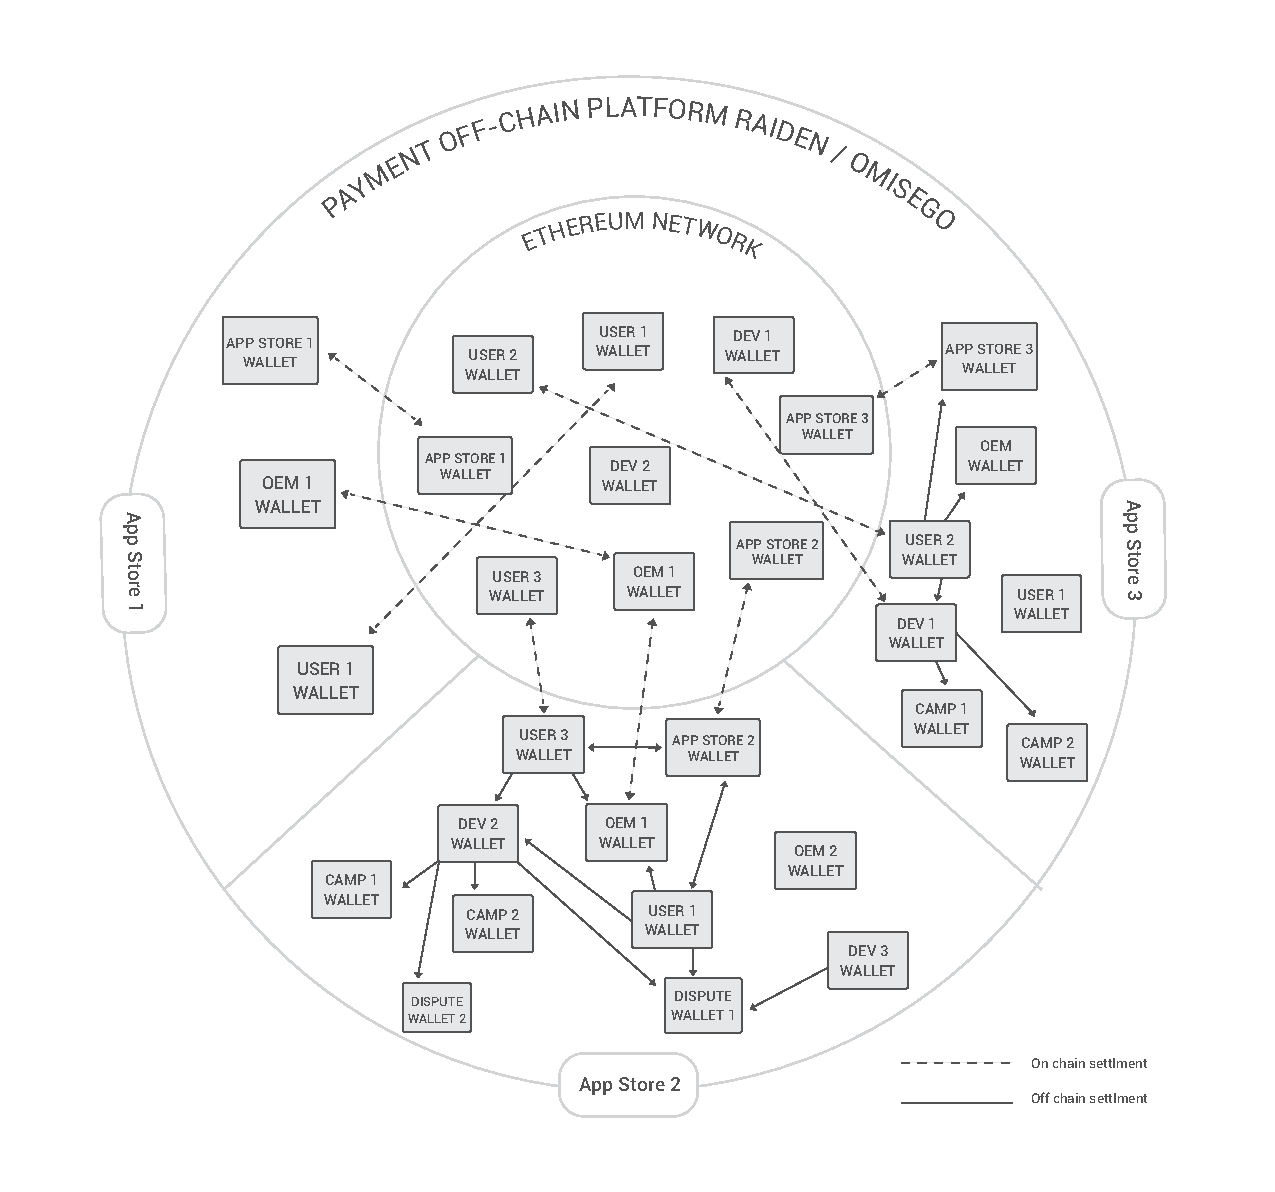
\includegraphics[width=\textwidth]{diagrams/offchain_wallets.eps}
\caption{On-chain and off-chain transactions.}
\label{fig:offchain}
\end{figure}


As seen in the previous section, there are blockchain currencies that can securely store digital value. But as we have seen, doing transactions over them does not scale, is slow and requires fees. Therefore alternatives like direct payment channels have to be evaluated.

In general terms, the App Store acts as the gateway to the digital payment world for the user. He deposits his valuables (preferably Ether) with the store in a payment channel using a smart contract. The same happens for developers. And from this moment on they can utilise the micro-payments within the App Infrastructure. The payments are instant, cheap and there can be any number of them.

The user has to pay fees on each Ether deposit to his account with the App Store and on checking out i.e. settling his payment channel. Further fees may be the taxation done by the App Store used to pay for its infrastructure.  If there are several App Stores in the same ecosystem like we envision, there might be further (minimal) fees to forward the payments from one to another.

Figure \ref{fig:offchain} depicts what is on-chain a vision of the wallets on-chain (Ethereum network) and the wallets off-chain using Raiden or OmiseGO.

% TODO explain better the division

Returning to the requirements from the beginning of this chapter, we plan to use Ethereum for storing value and smart contracts. 

To have scalability, Raiden is being evaluated for the first Beta version of the reference implementation of the protocol that is due six months after the ICO. %could not understand sentence

The choice for Raiden is because - at the time of writing - it is the only platform that has a test network and can be used. Yet OmiseGO has a promising outlook and in the future can be adopted depending on their progress. They will be kept under close look as they might develop the potential to substitute Raiden.






\section{Related Work}

This section presents the projects that inspired the AppCoins protocol solution to some extend, either because of the technology employed or by presenting concepts that underly the ones in our proposal. We first give a brief overview of each project and after we explain how each of our uses cases benefits from the contributions of each of the projects.

\subsection{Related Projects}
\subsubsection{Basic Attention Token}

The BAT project aims to revolutionise the digital advertising landscape by proposing a "decentralised, transparent digital ad exchange based on Blockchain" \textbf{[REF BAT PAPER]}. Their proposal is constituted by two components:
\begin{itemize}
	\item Brave: a browser that blocks third-party ads and trackers, which decreases webpages load time and ensures anonymity, while also building a ledger system that tracks users attention to ads in order to correctly reward publishers and advertisers
	\item BAT: a token for the decentralised ad exchange, connecting advertisers, publishers and users, while rewarding users for their attention
\end{itemize}

In their proposal, they want to eliminate the middlemen between advertisers and publishers, pay for user attention instead of CPM/clicks, provide faster webpage loads and ads tuned to user preferences, amongst other advantages. \\

By taking out the middlemen, they avoid the draining of resources by agencies, DSPs, exchanges, ad networks, and others, while also eliminating part of the complexity of having to handle with this huge ecosystem that is in place today. The gain in resources by eliminating the resource-draining players enables the sharing of resources by the important players in the flow: advertisers, publishers and users. Since there are less resources being wasted in middlemen, there is more available to be employed in processes that increase the value to the end user. They also propose to use machine learning at the browser level to serve tailored ads to users, instead of serving ads with no value. In addition, users are rewarded by their attention, which the project states as the "rare quantity", since the information available is far greater that the available attention each user has to give. \\

Today, publishers are paid based on clicks on ads. BAT proposes to start rewarding publishers based on the attention users give to ads, by keeping track of the user attention on a ledger system implemented in Brave, while always maintaining users' anonymity. User attention, as a very valuable asset, is not being rewarded correctly and users do not get anything while they navigate webpages and see the ads. The solution proposes that users also start receiving rewards for time spent seeing the ads while navigating, based on the amount of time they spend looking at them. \\

In order to reduce fraud, they propose approaches - calling them basic attention metrics (BAM) - to correctly identify users paying attention to ads. When the user attention is identified, it is saved in an anonymous way, while also ensuring that users do not get rewarded by paying attention to the same ad more that once. They define a \textit{proof-of-attention}, which ensures that a user can only see and get attributed to an ad once and maintains users' anonymity. This is achieved by using \textsf{ANONIZE} \textbf{[REF ANONYZE PAPER]} algorithm in a first stage. According to the authors, the algorithm is "the first implementation of a provably-secure multiparty protocol that scales to handle millions of users".  The BAT team says that they may also invest into using algorithms such as BOLT \textbf{[REF BOLT PAPER]}, zkSNARKs \textbf{[REF SNARKs PAPERS]} and STARKs \textbf{[REF STARKs PAPER]} to protect users' privacy.

\subsubsection{Kin}

The Kin project intends to create the "first open and sustainable alternative ecosystem of digital services
for our daily lives" \textbf{[REF KIN PAPER]}. In order to achieve this, a new cryptocurrency Kin is created to be used within the new ecosystem by the digital services. \\

Since Kin is being developed by Kik, a popular chat app with already millions of users, Kik will integrate Kin to showcase the possibilities of having an ecosystem of connected digital services. New partners joining the ecosystem will create a network effected, boosting the value of Kin. Kik will develop two main components of the new ecosystem:
\begin{itemize}
	\item Kin Reward Engine
	\item Kin Foundation
\end{itemize}

The Kin Reward Engine is going to create incentives for other digital services to adopt Kin. The majority of the Kin supply will be allocated to Kin Reward Engine and periodically will unlock and distribute a certain amount of Kin amongst the digital services within the ecosystem. The amount each digital service receives depends on the amount of Kin used by them. \\

Kin Foundation is the entity that will oversee the growth of the ecosystem, as well as administer the Kin Reward Engine. In time, the Kin Foundation will transition the entire ecosystem, including the Kin Reward Engine to a fully decentralised and autonomous network. When this happens, Kin Foundation main responsabilities will be helping onboarding new partners and overseeing development of fundamental components such as identity and reputation management, cryptocurrency wallets, and compliance solutions. \\

In the end, Kin wants to develop an ecosystem that is open and fair, where users benefit from a vast and diverse digital experience, being able to transition between services with almost no effort. Providers will be able to compete for compensation within the ecosystem.

\subsubsection{Monetha}

The Monetha project aims to change how e-commerce is done and how merchants can reach customer by "creating a universal decentralised trust and reputation solution working flawlessly together with mobile payments processing on the Ethereum blockchain leveraging smart contract technology" \textbf{[REF MONETHA PAPER]}. \\

Currently, merchants wanting to sell online face two options: creating their own website or joining the big marketplaces, such as Amazon, Ebay, Alibaba, etc. The former requires a very significant investment in brand creation and advertising in order to have customers going directly to their site. This is due to the fact that customers tend to buy on places they trust and that have good reputation. If there is a merchant with a website no-one has heard about, there will be a trust barrier for the customers. On the other hand, joining big marketplaces has the advantage of not needing much advertising and branding but there is still the need to create reputation and trust amongst customers. Merchants accomplish this by providing high quality products delivered within the agreed time and, in turn, receive positive reviews. The problem with this approach is that the reputation a merchant is able to build on one marketplace is not transferable to others. If a merchant wants to sell on several marketplaces, since they are all disconnected, the merchant needs to build a reputation amongst customers on all of them.

In addition to the reputation problem, big marketplaces also impose very complex transaction processes. The transactions settlements are troublesome to the customer due to the high number of steps required, which Monetha states that can go up to 16. An additional problem is the high transaction fees, both regarding the number of fees, with Monetha claiming that can go up to 15, and the amount needed to be paid by the merchant. High fees can deter a merchant with small margins to sell products in the marketplaces, leaving the merchant with the option to create a brand and website, which is also an expensive option as explained above. Not only merchants need to pay high fees but there is also long transaction times between the marketplace and the merchant. Since there are so many parties involved in a transaction, the settlement can take up to 3 days, or a week for international payments. Moreover, marketplaces often hold payments for a week because of the high probability of chargebacks.

Monetha proposes a solution composed by a decentralised trust and reputation system together with payments powered by blockchain technology using Ethereum. Instead of having marketplaces with their own reputation system, Monetha proposes that merchants in the network build their reputation from transactions, claims and reviews. Furthermore, the since the network is shared by all merchants, it is as if the network would be a huge marketplace where any customer can see the reputation and trust score of every merchant and vice-versa. Instead of having to build reputation in several different systems, their reputation is build automatically and available to everyone.

Since payments are done through Ethereum, settlements are much simpler and the connection is direct between the merchant and the customer. With fewer steps in the settlement comes the advantage of smaller settlement times, with the merchant getting the money within just a few minutes. Fees are also much smaller, with a fixed cost of 1.5\% of transaction fee. Finally, since there is no centralised marketplace, there is also no holding of payments.

\subsection{Projects Contributions}
\subsubsection{Advertising}

The Advertising use case, as described in section \textbf{[REF SECTION PAPER]}, states that in App Stores there are too many resource-draining middlemen, and the risk of fraud is too high because of the complexity of systems in place today. We

\subsubsection{IAB}

\subsubsection{Developers Reputation}








%\section{Future Work}

%(where we can include what is not yet addressed and how we see the evolution)


%\section{Acknowledgements}

% (Where we give credit to other people in the team and externaly that contributed to the document)

\bibliography{appcoins_whitepaper}

\end{document}
